\begin{beginningnote}
    Si tenga presente che alcuni termini utilizzati nel documento riportano la lettera \textbf{G} in apice, allo scopo di evidenziare le parole che assumono uno specifico significato nell'ambito del progetto. 
    Per comprenderle in maniera corretta, si rimanda il lettore al documento ``Glossario", che contiene un elenco completo di tutte le terminologie utilizzate con relative definizioni, 
    allo scopo di costruire un linguaggio uniforme che possa migliorare la comunicazione tra i componenti interni al gruppo e gli stakeholders\textsuperscript{G} esterni.   
\end{beginningnote}

%%%%%%%%%%%%%%%%%%%%%%%%%%%%%%%%%%%
% INTRODUZIONE
%%%%%%%%%%%%%%%%%%%%%%%%%%%%%%%%%%%
\section{Introduzione}\label{sec:introduzione}
\subsection{Scopo del documento}\label{sec:introduzione:scopo_del_documento}
Il presente documento ha lo scopo di descrivere nel dettaglio i componenti utilizzati e le scelte progettuali adottate per la realizzazione completa del progetto.
Verranno quindi trattati in dettaglio gli aspetti fondamentali riguardanti i requisiti necessari per il prodotto, le tecnologie adottate, i design pattern applicati, l'architettura logica e quella di deployment del prodotto.
Si intende fornire il ragionamento e le disposizioni per lo sviluppo del progetto, in modo da garantire coerenza con i requisiti specificati nel documento \textit{Analisi dei requisiti v5.0.0}. 

\subsection{Scopo del progetto}\label{sec:introduzione:scopo_del_progetto}
Il progetto nasce nell'ambito dei \textbf{sistemi gestionali di magazzino}, meglio noti con il termine inglese di \textit{Warehouse Management Systems} (WMS), con 
l'obiettivo di risolvere una serie di problematiche derivanti dalle soluzioni tradizionali tuttora presenti sul mercato.\\
Il focus principale sarà migliorare la user experience, tramite la realizzazione di un applicativo che proponga all'utente un'interazione con il magazzino in un 
ambiente di lavoro 3D. \\
Tale soluzione, rispetto ai tradizionali sistemi 2D, garantirebbe una maggiore comprensione degli spazi, proponendo una visualizzazione più intuitiva e completa 
degli spazi di magazzino. Permetterebbe quindi all'utente di prendere decisioni in modo più efficace ed efficiente, permettendo così di ottimizzare i processi di logistica.

Per raggiungere questo obiettivo, l'ambiente di lavoro non può essere una semplice visualizzazione del magazzino. L'utente dovrà infatti poter:
\begin{itemize}
    \item Spostarsi all'interno dell'ambiente 3D;
    \item Progettare le scaffalature che sono presenti nel magazzino e modificarle nel tempo;
    \item Simulare i flussi di movimento di prodotti.
\end{itemize}

Il progetto deve concretizzarsi nella realizzazione di una web app fruibile agli impiegati d'ufficio ed incentrata sulla visualizzazione 3D del magazzino.
Per visionare il capitolato\textsuperscript{G} completo e la documentazione del gruppo, si veda la sezione \hyperref[sec:ref_esterni]{Riferimenti Esterni} 
del documento.

%%%%%%%%%%%%%%%%%%%%%%%%%%%%%%%%%%%
% TECNOLOGIE
%%%%%%%%%%%%%%%%%%%%%%%%%%%%%%%%%%%
\section{Tecnologie}\label{sec:tecnologie}
In questa sezione si riportano gli strumenti e le tecnologie impiegati per lo sviluppo e l’implementazione del software relativo al progetto ``WMS3''.
Si riporta dunque una descrizione delle tecnologie e del linguaggio di programmazione utilizzato, nonché delle librerie e dei framework\textsuperscript{G} necessari.
L’obiettivo principale è garantire che il software sia sviluppato utilizzando le tecnologie più appropriate in termini di efficienza, efficacia ed affidabilità.

\subsection{Linguaggi e formato dati}
Per lo sviluppo e l'implementazione del software viene utilizzato il seguente linguaggio di programmazione.

\renewcommand{\arraystretch}{1.5}
\begin{xltabular}{0.98\textwidth}{|p{0.25\textwidth}|X|}
    \hline
    \multicolumn{2}{|c|}{\cellcolor{black}\textcolor{white}{\textbf{JavaScript (+ JSX)}}} \\
    \hline
    \cellcolor{gray!10} \textbf{Descrizione generale:} & JS è un linguaggio di programmazione ad alto livello interpretato e orientato agli eventi. Viene comunemente utilizzato per aggiungere interattività e dinamicità alle pagine web, ma può essere utilizzato anche per lo sviluppo di applicazioni web, mobile e desktop. JSX, invece, è un'estensione di sintassi per JS che consente di scrivere codice simile all'HTML all'interno di JavaScript, semplificando la definizione dei componenti UI e della loro struttura. JSX viene comunque trasformato in JS regolare durante il processo di compilazione.\\
    \hline
    \cellcolor{gray!10} \textbf{Utilizzo nel progetto:} & JS è il linguaggio di programmazione utilizzato per implementare la logica, gestire le interazioni dell'utente, gestire i contenuti dinamici nel progetto, nonché per il testing. JSX, nello specifico, viene utilizzato per semplificare e rendere più leggibile la codifica delle componenti dell'UI.\\
    \hline

    \caption{Linguaggi di programmazione utilizzati}
    \label{tab:linguaggi}
\end{xltabular}

\noindent Per quanto riguarda il formato dei dati vengono utilizzati i seguenti.
\begin{xltabular}{0.98\textwidth}{|p{0.25\textwidth}|X|}
    \hline
    \multicolumn{2}{|c|}{\cellcolor{black}\textcolor{white}{\textbf{JSON}}} \\
    \hline
    \cellcolor{gray!10} \textbf{Descrizione generale:} & JSON è un formato di scrittura (basato su JS) che si caratterizza per la sua grande leggibilità, dovuta ad una sintassi semplice e facilmente interpretabile dai computer. Viene utilizzato in diversi contesti, tra cui lo sviluppo web, le API di servizi web e lo scambio di dati tra applicazioni.\\
    \hline
    \cellcolor{gray!10} \textbf{Utilizzo nel progetto:} & Nel progetto, JSON viene utilizzato per memorizzare la configurazione del magazzino per poter, successivamente, ricostruire il magazzino semplicemente caricando il file .json. Viene inoltre utilizzato come formato dei messaggi scambiati tra componenti ed API.\\
    \hline
    \multicolumn{2}{|c|}{\cellcolor{black}\textcolor{white}{\textbf{SVG}}} \\
    \hline
    \cellcolor{gray!10} \textbf{Descrizione generale:} & SVG è un formato di file basato su XML utilizzato per descrivere grafica vettoriale bidimensionale. In particolare, consente di creare immagini scalabili senza perdita di qualità, adatte per essere visualizzate su dispositivi di diversi formati e dimensioni.\\
    \hline
    \cellcolor{gray!10} \textbf{Utilizzo nel progetto:} & Nel progetto, SVG viene utilizzato per configurare una planimetria personalizzata del magazzino. \\
    \hline
    
    \caption{Formato dei dati utilizzati}
    \label{tab:formato_dati}
\end{xltabular}

\subsection{Tecnologie implementative}
\begin{xltabular}{0.98\textwidth}{|p{0.25\textwidth}|X|}
    \hline
    \endhead
    \multicolumn{2}{|c|}{\cellcolor{black}\textcolor{white}{\textbf{Node.js (con npm) }}} \\
    \hline
    \cellcolor{gray!10} \textbf{Versione:} & v21.4.0\\
    \hline
    \cellcolor{gray!10} \textbf{Documentazione:} &  
        \begin{itemize}[topsep=0pt]
             \item Node.js: \url{https://nodejs.org/en/learn/getting-started/introduction-to-nodejs} \textcolor{gray}{\textit{(ultimo accesso 05-05-24)}}
            \item npm: \url{https://docs.npmjs.com/} \textcolor{gray}{\textit{(ultimo accesso 05-05-24)}}
        \end{itemize}\\
    \hline
    \cellcolor{gray!10} \textbf{Descrizione generale:} & Node.js è un framework JavaScript multipiattaforma e open-source tra i più utilizzati. In particolare, si tratta di un ambiente di esecuzione che permette di eseguire codice JavaScript come un qualsiasi linguaggio di programmazione, al di fuori dei browser. Invece, npm è il suo gestore di pacchetti predefinito.\\
    \hline
    \cellcolor{gray!10} \textbf{Utilizzo nel progetto:} & Viene utilizzato Node.js per la gestione back-end della web-app. Mentre, npm viene utilizzato come gestore di pacchetti per installare le dipendenze del progetto.\\
    \hline

    \multicolumn{2}{|c|}{\cellcolor{black}\textcolor{white}{\textbf{React.js}}} \\
    \hline
    \cellcolor{gray!10} \textbf{Versione:} & \textasciicircum v18\\
    \hline
    \cellcolor{gray!10} \textbf{Documentazione:} &  
         \url{https://react.dev/learn} \textcolor{gray}{\textit{(ultimo accesso 05-05-24)}} \\
    \hline
    \cellcolor{gray!10} \textbf{Descrizione generale:} & Si tratta di una libreria open-source per la creazione di interfacce utente in JavaScript. Utilizza il concetto di componentizzazione e il Virtual DOM per migliorare le prestazioni. \\
    \hline
    \cellcolor{gray!10} \textbf{Utilizzo nel progetto:} & Viene utilizzata questa libreria per creare le varie componenti dell'UI in quanto particolarmente adatta allo sviluppo di componenti riutilizzabili e dinamiche, con dati variabili nel tempo.\\
    \hline

    \multicolumn{2}{|c|}{\cellcolor{black}\textcolor{white}{\textbf{Next.js}}} \\
    \hline
    \cellcolor{gray!10} \textbf{Versione:} & v14.1.3\\
    \hline
    \cellcolor{gray!10} \textbf{Documentazione:} &  
         \url{https://nextjs.org/docs} \textcolor{gray}{\textit{(ultimo accesso 05-05-24)}} \\
    \hline
    \cellcolor{gray!10} \textbf{Descrizione generale:} & Next.js è un framework open-source che permette di costruire e distribuire rapidamente applicazioni su larga scala e pronte per la produzione, renderizzandole lato server. In particolare, si basa ed estende la libreria JavaScript React e utilizza Node.js come ambiente run-time.\\
    \hline
    \cellcolor{gray!10} \textbf{Utilizzo nel progetto:} & Next.js viene utilizzato per migliorare le funzionalità di React fornendo una struttura e degli strumenti che ne migliorano le prestazioni. Nello specifico, per creare la struttura dell'applicazione, implementare le API e gestire il routing. A tal proposito, si precisa l'utilizzo dell'app router per gestire la navigazione tra le diverse viste all'interno dell'app.\\
    \hline

     \multicolumn{2}{|c|}{\cellcolor{black}\textcolor{white}{\textbf{Three.js}}} \\
    \hline
    \cellcolor{gray!10} \textbf{Versione:} & \textasciicircum v0.162.0\\
    \hline
    \cellcolor{gray!10} \textbf{Documentazione:} &  
          \url{https://threejs.org/docs/index.html\#manual/en/introduction/Creating-a-scene} \textcolor{gray}{\textit{(ultimo accesso 05-05-24)}} \\
    \hline
    \cellcolor{gray!10} \textbf{Descrizione generale:} & Three.js è una libreria JavaScript open-source utilizzata per la realizzazione di contenuti 3D per il Web. In particolare, utilizza le API WebGL per integrare ambienti 3D a siti web usando un semplice canvas HTML.\\
    \hline
    \cellcolor{gray!10} \textbf{Utilizzo nel progetto:} & Fortemente consigliata dall'azienda proponente, questa libreria viene utilizzata per lo sviluppo della parte 3D del progetto.\\
    \hline

     \multicolumn{2}{|c|}{\cellcolor{black}\textcolor{white}{\textbf{React-three/fiber}}} \\
    \hline
    \cellcolor{gray!10} \textbf{Versione:} & \textasciicircum v8.15.19\\
    \hline
    \cellcolor{gray!10} \textbf{Documentazione:} &  
          \url{https://docs.pmnd.rs/react-three-fiber/getting-started/introduction} \textcolor{gray}{\textit{(ultimo accesso 05-05-24)}} \\
    \hline
    \cellcolor{gray!10} \textbf{Descrizione generale:} & React Three Fiber (R3F) è un React renderer per Three.js. Esso permette di costruire componenti, basati sulla logica 3D di Three.js, che siano riutilizzabili e indipendenti.\\
    \hline
    \cellcolor{gray!10} \textbf{Utilizzo nel progetto:} &  Viene utilizzato R3F per integrare al meglio Three.js con React. \\
    \hline

    \multicolumn{2}{|c|}{\cellcolor{black}\textcolor{white}{\textbf{React-three/drei}}} \\
    \hline
    \cellcolor{gray!10} \textbf{Versione:} & \textasciicircum v9.102.6 \\
    \hline
    \cellcolor{gray!10} \textbf{Documentazione:} &  
          \url{https://github.com/pmndrs/drei} \textcolor{gray}{\textit{(ultimo accesso 05-05-24)}}    \\
    \hline
    \cellcolor{gray!10} \textbf{Descrizione generale:} & Drei è semplicemente una raccolta di ``astrazioni già pronte all'uso'', ovvero di componenti generici basati su R3F che sono già completamente funzionali.\\
    \hline
    \cellcolor{gray!10} \textbf{Utilizzo nel progetto:} &  Viene utilizzato per integrare al meglio Three.js con React, semplificando e velocizzando lo sviluppo di alcune componenti 3D. \\
    \hline

    \multicolumn{2}{|c|}{\cellcolor{black}\textcolor{white}{\textbf{Zustand}}} \\
    \hline
    \cellcolor{gray!10} \textbf{Versione:} & \textasciicircum v4.5.2\\
    \hline
    \cellcolor{gray!10} \textbf{Documentazione:} &  
          \url{https://docs.pmnd.rs/zustand/getting-started/introduction} \textcolor{gray}{\textit{(ultimo accesso 05-05-24)}} \\
    \hline
    \cellcolor{gray!10} \textbf{Descrizione generale:} & Zustand è una libreria di gestione dello stato per React. Con un'API semplice e intuitiva, permette di gestire lo stato dell'applicazione in modo efficiente, riducendo la complessità dello sviluppo e migliorando le prestazioni delle applicazioni React.\\
    \hline
    \cellcolor{gray!10} \textbf{Utilizzo nel progetto:} & Viene utilizzata per una gestione efficiente, ma comunque semplice, dello stato tra le diverse componenti dell'applicazione. In particolare, per memorizzare lo stato corrente del magazzino, per la conversione tra stato e file di configurazione esterni, oltre che per gestire eventuali errori nella modifica dello stato stesso.\\
    \hline


    \multicolumn{2}{|c|}{\cellcolor{black}\textcolor{white}{\textbf{Ant Design}}} \\
    \hline
    \cellcolor{gray!10} \textbf{Versione:} & \textasciicircum v5.16.1\\
    \hline
    \cellcolor{gray!10} \textbf{Documentazione:} &  
          \url{https://ant.design/components/overview/} \textcolor{gray}{\textit{(ultimo accesso 05-05-24)}} \\
    \hline
    \cellcolor{gray!10} \textbf{Descrizione generale:} & Ant Design è una libreria di componenti UI React open-source. Offre una vasta gamma di componenti pronti all'uso per la creazione di interfacce utente moderne e intuitive. Semplifica così lo sviluppo di applicazioni web React e, al contempo, migliora l'aspetto estetico del prodotto finale.\\
    \hline
    \cellcolor{gray!10} \textbf{Utilizzo nel progetto:} & Vengono utilizzate le componenti di Ant Design per l'interfaccia grafica. Vengono anche utilizzate le icone fornite da Ant Design per migliorare l'intuitività delle funzionalità all'interno dell'UI.\\
    \hline

    \caption{Tecnologie implementative}
    \label{tab:tec_implementative}
\end{xltabular}

\subsection{Tecnologie per il testing}
\begin{xltabular}{0.98\textwidth}{|p{0.25\textwidth}|X|}
    \hline
    \endhead
    \multicolumn{2}{|c|}{\cellcolor{black}\textcolor{white}{\textbf{Jest}}} \\
    \hline
    \cellcolor{gray!10} \textbf{Versione:} & \textasciicircum v29.7.0\\
    \hline
    \cellcolor{gray!10} \textbf{Documentazione:} &  
            \url{https://jestjs.io/docs/getting-started} \textcolor{gray}{\textit{(ultimo accesso 05-05-24)}}\\
    \hline
    \cellcolor{gray!10} \textbf{Descrizione generale:} & Jest è un framework di testing JavaScript comunemente utilizzato per testare applicazioni React e Node.js. In particolare, offre funzionalità integrate per il mocking, l'esecuzione dei test in parallelo e la copertura del codice, migliorando l'affidabilità e la qualità del software. \\
    \hline
    \cellcolor{gray!10} \textbf{Utilizzo nel progetto:} & Viene utilizzato per l'implementazione di unit e integration test dell'applicazione, sia per la parte logica sia per l'interfaccia utente.\\
    \hline

    \multicolumn{2}{|c|}{\cellcolor{black}\textcolor{white}{\textbf{Testing-library/react}}} \\
    \hline
    \cellcolor{gray!10} \textbf{Versione:} & \textasciicircum v15.0.2\\
    \hline
    \cellcolor{gray!10} \textbf{Documentazione:} &  
         \url{https://testing-library.com/docs/} \textcolor{gray}{\textit{(ultimo accesso 05-05-24)}} \\
    \hline
    \cellcolor{gray!10} \textbf{Descrizione generale:} & React Testing Library è una libreria di testing per applicazioni React che si concentra sulla validazione dell'interazione dell'utente con l'applicazione. \\
    \hline
    \cellcolor{gray!10} \textbf{Utilizzo nel progetto:} & Viene utilizzata assieme a Jest per l'implementazione di test che riguardano componenti di React.js. Inoltre, si precisa l'utilizzo dei pacchetti aggiuntivi jest-dom e user-event per il miglioramento dell'affidabilità e leggibilità dei test.\\
    \hline

    \multicolumn{2}{|c|}{\cellcolor{black}\textcolor{white}{\textbf{React-three/test-renderer}}} \\
    \hline
    \cellcolor{gray!10} \textbf{Versione:} & \textasciicircum v8.2.1\\
    \hline
    \cellcolor{gray!10} \textbf{Documentazione:} &  
         \url{https://github.com/pmndrs/react-three-fiber/tree/master/packages/test-renderer} \textcolor{gray}{\textit{(ultimo accesso 05-05-24)}} \\
    \hline
    \cellcolor{gray!10} \textbf{Descrizione generale:} & È una libreria che semplifica il testing di componenti React che utilizzano Three.js per la grafica 3D. Consente di renderizzare e testare componenti 3D, simulare eventi utente e verificare lo stato e il comportamento dei componenti in risposta a interazioni simulate. \\
    \hline
    \cellcolor{gray!10} \textbf{Utilizzo nel progetto:} & Viene utilizzata assieme a Jest per l'implementazione di test che riguardano componenti 3D realizzate attraverso React-three/fiber e React-three/drei.\\
    \hline

    \caption{Tecnologie per il testing}
    \label{tab:tec_test}
\end{xltabular}

%% jest e react testing library

\subsection{Tecnologie per il deployment}
\begin{xltabular}{0.98\textwidth}{|p{0.25\textwidth}|X|}
    \hline
    \endhead
    \multicolumn{2}{|c|}{\cellcolor{black}\textcolor{white}{\textbf{Vercel}}} \\
    \hline
    \cellcolor{gray!10} \textbf{Versione:} & \textasciicircum v29.7.0\\
    \hline
    \cellcolor{gray!10} \textbf{Documentazione:} &  
            \url{https://vercel.com/docs} \textcolor{gray}{\textit{(ultimo accesso 05-05-24)}}\\
    \hline
    \cellcolor{gray!10} \textbf{Descrizione generale:} & Vercel è una piattaforma di hosting serverless per applicazioni web e siti statici. Integra anche funzionalità di deployment continuo e collaborazione in tempo reale.\\
    \hline
    \cellcolor{gray!10} \textbf{Utilizzo nel progetto:} & Viene utilizzato per una semplice distribuzione del software. In particolare, viene collegato il repository GitHub con il codice sorgente del progetto alla piattaforma. In tal modo, si ha un deployment automatico, garantendo dunque un aggiornamento continuo e senza problemi. \\
    \hline

    \caption{Tecnologie per il deployment}
    \label{tab:tec_deploy}
\end{xltabular}


%%%%%%%%%%%%%%%%%%%%%%%%%%%%%%%%%%%
% ARCHITETTURA LOGICA
%%%%%%%%%%%%%%%%%%%%%%%%%%%%%%%%%%%
\newpage
\section{Architettura logica}\label{sec:architettura_logica}
Il gruppo ha dato particolare attenzione alla scelta di un'architettura che favorisse una adeguata ``\textit{separation of concerns}", specialmente tra la logica di business e la logica di presentazione. Una corretta applicazione di questo principio porta, infatti, ad una maggior coesione e ad una riduzione dell'accoppiamento nel software.

Questa parte del documento esplorerà dunque i pattern adottati per raggiungere tale obiettivo e descriverà i componenti che ne derivano.

\subsection{Pattern}\label{sec:pattern_e_tecnologie}
Questa sezione ha lo scopo di illustrare le motivazioni e i pattern sui quali il gruppo si è basato per la progettazione. L'obiettivo è di fornire una migliore comprensione del significato di ciascun elemento software nel contesto dell'architettura applicata al progetto.

\subsubsection{Motivazioni e ispirazioni: studio delle tecnologie}
\par Di fatto, le tecnologie scelte non pongono particolari limitazioni sul pattern architetturale da applicare al progetto, perciò la scelta e l'implementazione sono lasciate al team di sviluppo. 

Tuttavia, alcuni pattern vengono considerati best practice e/o vengono suggeriti dalle risorse di riferimento delle tecnologie utilizzate. Ad esempio, per la libreria di gestione dello stato Zustand, utilizzata nel progetto, vengono raccomandati alcuni pattern ispirati alle architetture \textit{Flux} e \textit{Redux}. In realtà, è proprio la documentazione stessa dello strumento ad evidenziare la possibilità di utilizzare i principi \textit{Flux} nell'applicazione. Mentre, per quanto riguarda la gestione dell'UI con React.js, anch'esso utilizzato nel progetto, si adotta un'architettura a componenti, come suggerito dalla struttura stessa di React. Inoltre, viene consigliata l'adozione del pattern \textit{Container/Presentational}.

Per maggiori informazioni si rimanda alla sezione \hyperref[sec:ref_esterni]{Riferimenti Esterni} del documento.

\subsubsection{Le architetture Flux/Redux}
\paragraph{Descrizione del funzionamento}
L'architettura \textit{Flux} nasce come proposta alternativa alle varianti del pattern MVC sviluppate nel corso del tempo per la progettazione di applicazioni web client-side, in particolare con React. L'esigenza alla base di \textit{Flux} era far fronte ai problemi di dipendenze tra le componenti architetturali (legate attraverso un ``two-way data binding"), che potevano crescere di complessità, man mano che l'applicazione web cresceva di dimensione, con l'aggiunta, ad esempio, di nuovi modelli e nuove view a quelli già presenti.
\par La principale differenza che presenta \textit{Flux} è lo ``\textit{unidirectional data flow}", e cioè il flusso di dati segue un'unica direzione: nei pattern precedenti (derivati di MVC), i cambiamenti sulla view erano riportati al model e viceversa, ma con \textit{Flux} una modifica segue un unico flusso rigorosamente definito, descritto dal diagramma sottostante.
\begin{center}
    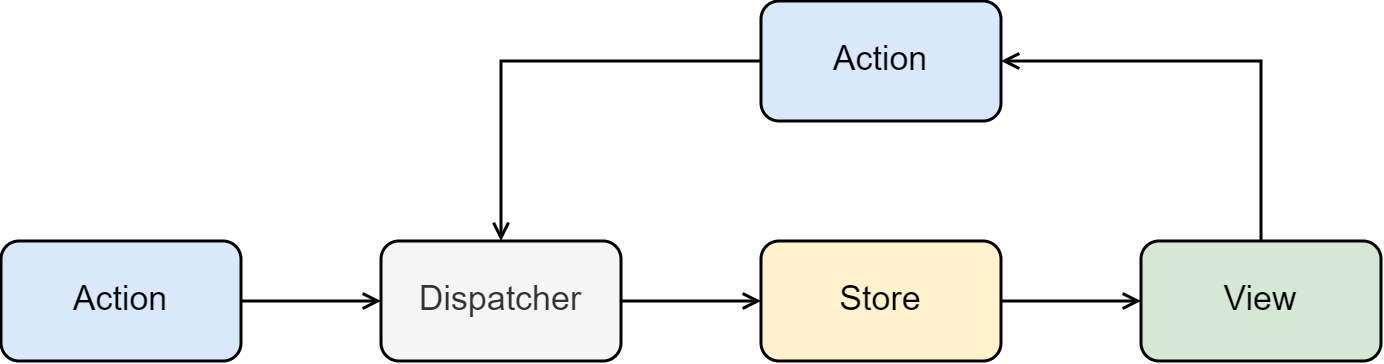
\includegraphics[scale=0.8]{images/flux.png}
\end{center}
\noindent Gli elementi dell'architettura sono:
\begin{itemize}
    \item \textbf{Store}: contiene lo stato e la logica dell'applicazione. Nella sua implementazione originale, possono esistere diversi store, ciascuno contenente informazioni su uno specifico dominio nell'applicazione;
    \item \textbf{Dispatcher}: funziona da hub centrale per l'applicazione e gestisce la distribuzione delle azioni agli stores;
    \item \textbf{View}: rappresenta l'interfaccia utente, gestisce la visualizzazione dei dati e l'interazione con l'utente. Gli elementi della view rimangono in ascolto per cambiamenti sugli store ed effettuano il re-render se necessario;
    \item \textbf{Actions}: sono oggetti che contengono le informazioni necessarie per compiere un'azione sullo stato dell'applicazione. Possiedono una proprietà \textit{type} che identifica il tipo di azione. Possono originarsi dalla view come risultato dell'interazione utente, ma anche dal server. 
\end{itemize}
\noindent Come si può vedere, una modifica può essere effettuata solo tramite actions, le quali entrano nello store attraverso il dispatcher. Quando lo stato nello store cambia, la view effettua un re-render automatico. Questo pattern ben si adatta alle tecnologie scelte, perché rispecchia il funzionamento di React ed aiuta a mantenere il sistema più consistente.
\par Un'evoluzione di \textit{Flux} è \textit{Redux}, che implementa il pattern applicando alcuni elementi della programmazione funzionale, pur mantenendo gli stessi concetti che stanno alla base del suo precursore. In particolare, \textit{Redux} si differenzia da \textit{Flux} per:
\begin{itemize}
    \item L'assenza del dispatcher, non necessario perché utilizza funzioni pure, che non hanno bisogno di ulteriori entità che le gestiscano;
    \item L'assunzione che le informazioni nello stato non vengano mai mutate, ma piuttosto che si crei un nuovo oggetto a partire dall'informazione iniziale;
    \item La presenza di un singolo store piuttosto che tanti, che quindi funge da ``unique source of truth".
\end{itemize}

\paragraph{L'implementazione con Zustand}
Come accennato in precedenza, Zustand è per sua natura``unopinionated", tuttavia è possibile (e raccomandato) costruire una struttura che mantiene i concetti delle architetture \textit{Flux} e \textit{Redux}. 

Zustand riesce anche a semplificare l'utilizzo di queste, in quanto sfrutta gli hooks di React per realizzare lo state management. Nello specifico, per come è implementata la libreria, non è necessario l'utilizzo di un dispatcher o dei reducer dell'architettura \textit{Redux}. Infatti, tramite appunto l'utilizzo degli hooks, è possibile ottenere un comportamento ``flux-like" senza l'utilizzo di ulteriori elementi nell'architettura.

Ed è proprio attraverso questa soluzione che il gruppo ha deciso di basare la progettazione del prodotto finale, utilizzando un'architettura che rispecchia gli standard moderni per le tecnologie scelte, pur mantenendo i vantaggi offerti dalla libreria Zustand. Infatti, oltre a tutto ciò, Zustand offre anche vantaggi in termini di leggibilità e semplicità della sintassi, leggerezza della gestione dello stato, nonché consente l'utilizzo di funzioni puramente JavaScript per definire le azioni di stato.

\paragraph{Adozione del pattern nel progetto}
Gli elementi che compongono il pattern adottato per l'architettura del progetto sono elencati di seguito, ciascuno con una breve spiegazione.
\begin{itemize}
    \item \textbf{Store}: è la componente unica che contiene lo stato globale dell'applicazione, rappresentando una ``\textit{single source of truth}". Lo store contiene dati (sotto forma di tipi primitivi ed oggetti) ed azioni. Seguendo lo \textit{slices pattern}, uno store può essere composto da più slices.
    \item \textbf{Slices}: sono unità individuali che rappresentano un sottoinsieme dello stato globale dell'applicazione, permettendo una migliore modularità nello state management. È bene che una slice contenga dati ed azioni che fanno riferimento ad uno specifico dominio dell'applicazione.
    \item \textbf{Actions}: sono funzioni contenute nelle slices e rappresentano l'unico modo di operare sui dati contenuti nello store. All'interno di una action, si utilizza la funzione \textit{set} per aggiornare lo stato nello store, che effettua un merge in maniera automatica, mantenendo il principio di immutabilità.
    \item \textbf{View}: rappresenta l'interfaccia grafica del progetto e gestisce l'interazione con l'utente. È composta da diversi componenti React, ciascuno dei quali può effettuare l'operazione di ``subscribe" ad un particolare sottoinsieme dello stato globale e, in questo caso, il re-render viene effettuato in maniera automatica solo al cambiamento di quella particolare pozione dello stato. Sempre attraverso la view, è possibile chiamare le actions delle slices per aggiornare lo stato dell'applicazione.
\end{itemize}

\subsubsection{L'architettura a componenti e il pattern Container/Presentational}
\paragraph{Descrizione del funzionamento}
Nel contesto dello sviluppo di interfacce utente moderne, l'architettura a componenti è diventata uno standard comune. Essa si basa sul concetto di suddividere l'interfaccia utente in componenti (i.e. unità autonome) riutilizzabili e modulari. Ogni componente è infatti responsabile di una specifica parte dell'interfaccia e può contenere sia la logica di presentazione che la logica di gestione dei dati.

Un approccio comune per organizzare i componenti è il pattern \textit{Container/Presentational}. Questo pattern prevede la separazione dei componenti in due categorie principali:
\begin{itemize}
    \item \textbf{Componenti Container:} questi componenti sono responsabili della gestione dei dati e della logica di business dell'applicazione. Essi, infatti, si occupano di recuperare i dati da una fonte esterna, elaborarli e passarli ai componenti Presentational. Sono spesso connessi allo stato dell'applicazione e possono utilizzare i metodi di gestione dello stato per aggiornare dinamicamente l'interfaccia utente.
    \item \textbf{Componenti Presentational:} questi componenti sono responsabili dell'aspetto visivo dell'applicazione e della visualizzazione dei dati forniti loro dai componenti Container. Essi, infatti, non contengono logica di business o di gestione dei dati, bensì si concentrano esclusivamente sulla presentazione dei dati all'utente in modo chiaro e comprensibile.
\end{itemize}
Riassumendo, in un'architettura basata sul pattern \textit{Container/Presentational}, il componente container gestisce la logica di business, mentre il componente presentazionale si occupa solo dell'aspetto visivo dei dati. 

Questo approccio promuove dunque la separazione dei concetti e aderisce al principio di singola responsabilità. Ciò porta ad una maggiore leggibilità, riutilizzabilità e modularità del codice, semplificando anche il processo di testing. Inoltre, questa netta separazione consente di aggiungere e rimuovere componenti presentazionali senza influenzare la logica dell'applicazione, rendendo il sistema più scalabile e facile da mantenere.

\paragraph{Implementazione con React.js}
React.js offre un set di strumenti e convenzioni che facilitano l'utilizzo di questa architettura.
\begin{itemize}
    \item \textbf{Componenti React:} i componenti sono il fondamento dello sviluppo dell'interfaccia utente in React. In particolare, ogni componente React è una funzione o una classe che restituisce un'interfaccia utente sotto forma di elementi React. È possibile anche strutturare più componenti in un albero gerarchico per creare interfacce utente più complesse.
    \item \textbf{Props e State:} React utilizza props e state per consentire la comunicazione tra i componenti e per gestire lo stato dell'applicazione. Le props sono passate da un componente genitore a un componente figlio e vengono utilizzate per trasmettere dati e configurazioni. Lo state è un oggetto locale a ciascun componente e viene utilizzato per gestire le informazioni dinamiche all'interno di quel componente.
    \item \textbf{Hook di React:} gli hook di React consentono ai componenti funzionali di utilizzare lo state e altre funzionalità di React. 
\end{itemize}
Dunque, con riferimento all'architettura a componenti, quest'ultime sono individuate dalle componenti di React stesse.
Per quanto riguarda il pattern \textit{Container/Presentational}, questo è implementato in React tramite:
\begin{itemize}
    \item l'utilizzo degli hook di React nelle componenti Container per gestire lo stato dell'applicazione e gli effetti collaterali;
    \item l'utilizzo delle props (ricevuti dai componenti Container) nelle componenti Presentational per renderizzare l'UI in base a tali dati.
\end{itemize}

\paragraph{Adozione del pattern nel progetto}
Nel nostro progetto, abbiamo adottato l'architettura a componenti e il pattern \textit{Container/Presentational} per organizzare la parte ``View'' del sistema. Nello specifico, i componenti Container accedono allo store di Zustand, ricevono dati dalla componente Presentational (tramite funzioni passati come props) e li aggiornano nello store. D'altra parte, i componenti Presentational mostrano i dati ricevuti come props dai componenti Container e trasmettono, a loro volta, i dati ricevuti dall'utente ai componenti Container.

Questo approccio ci ha dunque permesso di separare chiaramente la logica di gestione dei dati dalla logica di presentazione, migliorando la chiarezza e la manutenibilità del nostro codice. 

\subsection{Descrizione dell'architettura}
Si riportano di seguito i diagrammi UML delle classi e delle componenti del sistema, corredati da una descrizione che ne chiarisce il significato e la funzionalità. 

Per facilitare la comprensione dei diagrammi si utilizzano diversi colori per indicare un diverso tipo di entità:
\begin{itemize}
    \item \colorbox{rosso_uml}{\textbf{Rosso:}} store e slices. In particolare, con riferimento ad un singolo elemento di questi:
        \begin{itemize}
            \item \colorbox{giallo_uml}{\textbf{Giallo:}} per uno stato,
            \item \colorbox{viola_uml}{\textbf{Violetto:}} per un'action;
        \end{itemize}
    \item \colorbox{verde_uml}{\textbf{Verde:}} componenti React;
    \item \colorbox{azzurro_uml}{\textbf{Azzurro}:} classi di modello e oggetti.
\end{itemize}

Si noti inoltre che i metodi \textit{setter} e \textit{getter} per campi privati vengono omessi dai diagrammi per mantenere chiarezza e leggibilità degli stessi, concentrando l'attenzione su aspetti più rilevanti.

\subsubsection{Store e model} 
Nel diagramma sottostante vengono mostrate dipendenze dello store, incluse tutte le slice e le componenti React che accedono a queste slice tramite lo store. Vedremo in dettaglio le componenti React nella sezioni \ref{sec:uml_react}, mentre in questa sezione approfondiremo, invece, la parte di modello e composizione dello store stesso.
\begin{figure}[H]
    \centering
    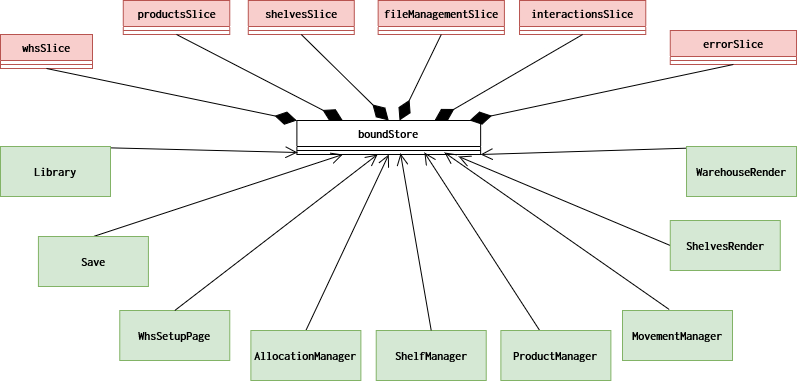
\includegraphics[width=\textwidth]{images/UML/feature_model_general.drawio.png}
    \label{fig:UML_model}
    \caption{Diagramma UML delle dipendenze dello store}
\end{figure}

Lo store, denominato \textbf{boundStore}, agisce come un contenitore per lo stato globale dell'applicazione, il quale viene composto dalle varie slice definite. Infatti, ogni slice rappresenta una parte specifica dello stato che ha pertinenza su un certo dominio dell'applicazione.

\bigskip
\noindent Si esamina di seguito la composizione di ciascuna slice. 

\paragraph{Slice whsSlice}
\begin{figure}[H]
    \centering
    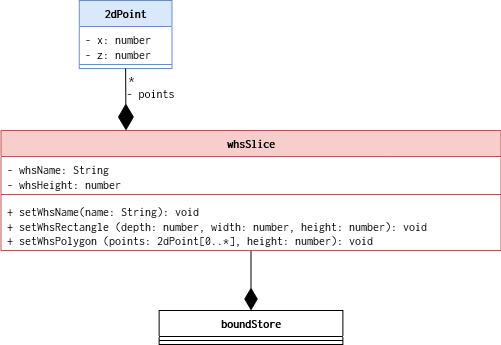
\includegraphics[width=0.8\textwidth]{images/UML/feature_model_whsSlice.drawio.png}
    \label{fig:UML_whsSlice}
    \caption{Diagramma UML della whsSlice}
\end{figure}
Questa slice contiene informazioni sullo stato del magazzino di per sé, in particolare contiene:
\begin{itemize}
    \item il nome identificativo (\textbf{whsName}); 
    \item le dimensioni, rappresentate attraverso un semplice numero (\textbf{whsHeight}) per l'altezza e attraverso un array (\textbf{points}) di oggetti nel formato \textit{\{x, z\}} per indicare i vari punti di angolo del magazzino.
\end{itemize}

\noindent Le action contenute in questa slice sono invece:
\begin{itemize}
    \item \textbf{setWhsName} utilizzata per impostare il nome del magazzino;
    \item due funzioni per impostare le dimensioni del magazzino:
    \begin{itemize}
        \item \textbf{setWhsRectangle}, utilizzata nel caso in cui il magazzino sia creato di default, i.e. con planimetria rettangolare,
        \item \textbf{setWhsPolygon}, utilizzata nel caso in cui il magazzino sia creato con planimetria personalizzata (poligonale).
    \end{itemize}
\end{itemize}
Nel caso di successo di un'action, viene aggiornato correttamente lo stato, altrimenti viene impostato un errore nella errorSlice.


\paragraph{Slice shelvesSlice}
\begin{figure}[H]
    \centering
    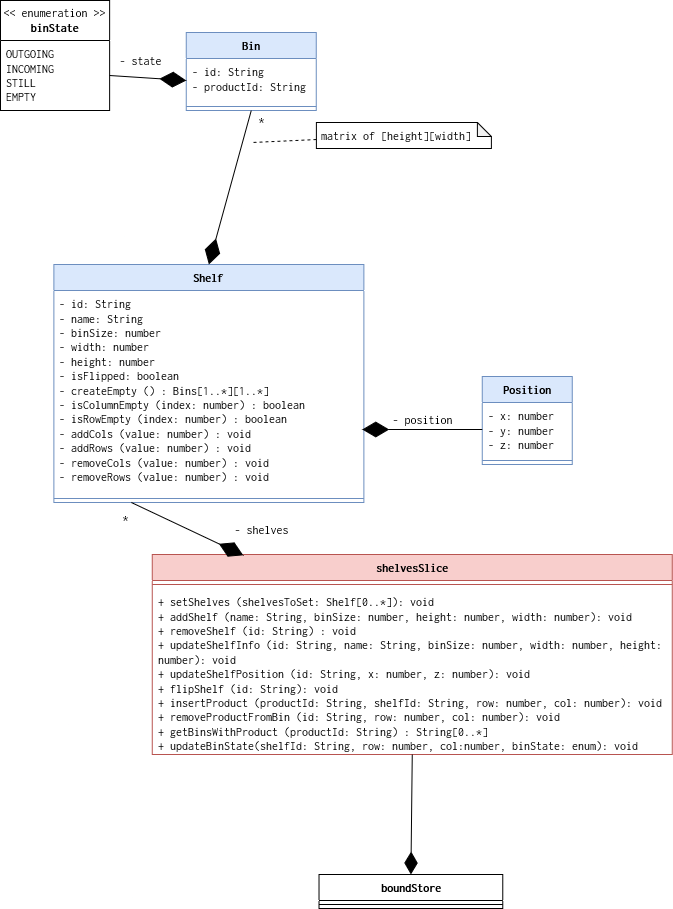
\includegraphics[width=\textwidth]{images/UML/feature_model_shelvesSlice.drawio.png}
    \label{fig:UML_shelvesSlice}
    \caption{Diagramma UML della shelvesSlice}
\end{figure}
Questa slice contiene le informazioni sullo stato delle scaffalature, in particolare possiede un elenco delle scaffalature (\textbf{shelves}) contenute nel magazzino. 

Le scaffalature sono rappresentate individualmente come oggetti della classe ``Shelf'', la quale raggruppa in sé tutte le informazioni di una scaffalatura, ovvero:
\begin{itemize}
    \item elementi identificativi, quali \textbf{id} univoco (nella forma s\_[uuid]) e \textbf{nome};
    \item dimensioni, ovvero misura dei bin\textsuperscript{G} (\textbf{binSize}) e numero di questi in altezza (\textbf{height}) e larghezza (\textbf{width});
    \item disposizione della scaffalatura nel magazzino, i.e. la sua posizione (\textbf{position}, rappresentata da un oggetto del tipo \textit{\{x,y,z\}}) e orientamento (\textbf{isFlipped});
    \item occupazione della scaffalatura, attraverso una matrice di oggetti ``Bin''. Ciascuno di questi indica lo stato del prodotto contenuto nel bin (\textbf{state}) e, se presente, l'id del prodotto (\textbf{productId}) contenuto in essi. Questi ``Bin'' vengono identificati da un \textbf{id} univoco formato da [id di Shelf]+[row]+[col], dove ``row'' e ``col'' sono gli indici della matrice relativi al bin in questione.
\end{itemize}
Questa classe ``Shelf'' fornisce anche tutta una serie di funzioni (visibili nel diagramma sovrastante) che servono a modificare le dimensioni della matrice di oggetti ``Bin'' ed, eventualmente, generare errori in caso ciò non sia possibile.

\bigskip
\noindent Le action contenute in shelvesSlice sono invece:
\begin{itemize}
    \item \textbf{setShelves}, utilizzato per impostare direttamente shelves. In particolare, viene impiegato durante la configurazione del magazzino da file, quando possono essere presenti più scaffalature;
    \item \textbf{addShelf} e \textbf{removeShelf}, utilizzate rispettivamente per aggiungere e rimuovere una scaffalatura dallo stato;
    \item \textbf{updateShelfInfo}, \textbf{updateShelfPosition} e \textbf{flipShelf} utilizzate per aggiornare i diversi dati relativi alla configurazione di una scaffalatura;
    \item \textbf{insertProduct}, \textbf{removeProductFromBin} e \textbf{updateBinState} per gestire l'inserimento e rimozione di prodotti dai bin della scaffalatura;
    \item \textbf{getBinsWithProduct}, per ottenere una panoramica di tutti i bin presenti nel magazzino che contengono un determinato prodotto.
\end{itemize}
Nel caso di successo di un'action, viene aggiornato correttamente lo stato, altrimenti viene impostato un errore nella errorSlice.

\paragraph{Slice productsSlice}
\begin{figure}[H]
    \centering
    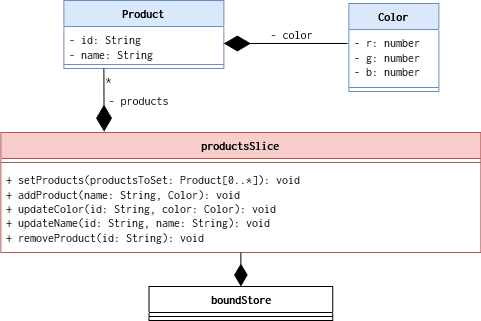
\includegraphics[width=0.8\textwidth]{images/UML/feature_model_productsSlice.drawio.png}
    \label{fig:UML_productsSlice}
    \caption{Diagramma UML della productsSlice}
\end{figure}
Questa slice contiene le informazioni sullo stato dei prodotti, in particolare possiede un elenco dei prodotti (\textbf{products}) che sono distribuiti nel magazzino.

I prodotti sono modellati come oggetti della classe ``Product'', la quale raggruppa in sé tutte le informazioni di un prodotto, ovvero:
\begin{itemize}
    \item elementi identificativi, quali \textbf{id} univoco (nella forma p\_[uuid]) e \textbf{nome};
    \item colore del prodotto, rappresentato da un oggetto nel formato \textit{\{r,g,b\}}.
\end{itemize}
Si tenga presente che questi oggetti rappresentano "etichette" più che prodotti fisici. Essi infatti possono esistere senza essere fisicamente nel magazzino, oppure posso essere presenti nel magazzino in una o più copie. Il singolo prodotto fisico è dunque simboleggiato dal contenuto di un determinato bin.

\bigskip
\noindent Le action contenute in productsSlice sono invece:
\begin{itemize}
    \item \textbf{setProducts}, utilizzato per impostare direttamente products. In particolare, viene impiegato durante la configurazione del magazzino da file, quando possono essere presenti più prodotti;
    \item \textbf{addProduct} e \textbf{removeProduct}, utilizzate rispettivamente per aggiungere e rimuovere completamente un prodotto dallo stato;
    \item \textbf{updateName} e \textbf{updateColor} utilizzate per aggiornare i diversi dati relativi ad un prodotto;
\end{itemize}
Nel caso di successo di un'action, viene aggiornato correttamente lo stato, altrimenti viene impostato un errore nella errorSlice.


\paragraph{Slice interactionsSlice}
\begin{figure}[H]
    \centering
    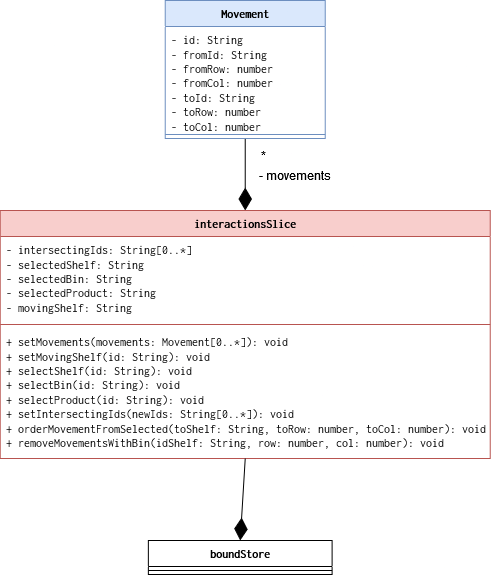
\includegraphics[width=0.8\textwidth]{images/UML/feature_model_interactionsSlice.drawio.png}
    \label{fig:UML_interactionsSlice}
    \caption{Diagramma UML dell'interactionsSlice}
\end{figure}
Questa slice contiene le informazioni sulle attuali interazioni dell'utente con il magazzino. In particolare contiene:
\begin{itemize}
    \item un array (\textbf{intersectingIds}) degli elementi del magazzino tra cui vi è una collisione causata, ad esempio, dal movimento di una scaffalatura;
    \item l'id dell'elemento attualmente selezionato (esclusivamente uno tra \textbf{selectedShelf}, \textbf{selectedBin} e \textbf{selectedProduct}, gli altri sono invece posti a \textit{null});
    \item l'id della scaffalatura (\textbf{movingShelf}) che è in movimento al momento (se presente);
    \item un array (\textbf{movements}) delle richieste di movimento (di prodotti) pendenti. 
        \begin{itemize}
            \item Una singola di queste richieste è rappresentata da un oggetto ``Movement'', identificato da un \textbf{id} (nel formato m\_[uuid]). Esso contiene le informazioni sull'attuale posizione del prodotto da movimentare (\textbf{fromId} , \textbf{fromRow} e \textbf{fromCol}, che nella forma [fromId]+[fromRow]+[fromCol] rappresentano il bin di origine) e sulla destinazione dopo il movimento, se completato con successo (\textbf{toId} , \textbf{toRow} e \textbf{toCol}, che nella forma [toId]+[toRow]+[toCol] rappresentano il bin di arrivo).
        \end{itemize}
\end{itemize}

\noindent Le action contenute in interactionsSlice sono invece:
\begin{itemize}
    \item \textbf{setMovements}, utilizzato per impostare direttamente movements. In particolare, viene impiegato durante la configurazione del magazzino da file, quando possono essere presenti più movimentazioni pendenti;
    \item \textbf{selectShelf}, \textbf{selectProduct} e \textbf{selectBin}, per impostare rispettivamente una scaffalatura, un prodotto o un bin come elemento correntemente selezionato e, al contempo, deselezionare qualsiasi altro elemento eventualmente già selezionato;
    \item \textbf{setMovingShelf}, per impostare una scaffalatura come ``in movimento'';
    \item \textbf{setIntersectingIds}, per segnalare tutti gli elementi correntemente interessati da una collisione;
    \item \textbf{orderMovementFromSelected} e \textbf{removeMovementsWithBin},  utilizzate rispettivamente per aggiungere e rimuovere un movimento di un prodotto dallo stato.
\end{itemize}
Nel caso di successo di un'action, viene aggiornato correttamente lo stato, altrimenti viene impostato un errore nella errorSlice.

\paragraph{Slice fileManagementSlice}
\begin{figure}[H]
    \centering
    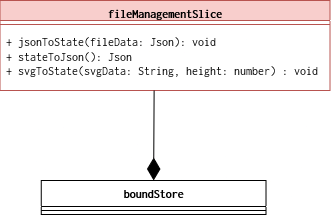
\includegraphics[width=0.6\textwidth]{images/UML/feature_model_fileManagement.drawio.png}
    \label{fig:UML_fileManagementSlice}
    \caption{Diagramma UML della fileManagementSlice}
\end{figure}
Questa slice funge da tramite tra le funzioni dello stato e i dati di configurazione in formato JSON ed SVG. In particolare, essa si occupa di ricevere i dati JSON e chiamare le funzioni appropriate dello stato per aggiornare le informazioni (attraverso l'action \textbf{jsonToState}). Viceversa, quando vi è la necessità di trasferire dati dallo stato al formato JSON, per salvare la configurazione del magazzino, questa slice si occupa di tale conversione (attraverso l'action \textbf{stateToJson}). Analogamente, gestisce anche la conversione dei dati dal formato SVG, utilizzato per planimetrie personalizzate del magazzino, allo stato (attraverso l'action \textbf{svgToState}).

Si noti che le funzioni all'interno di questa slice si occupano esclusivamente della conversione dei dati e dell'aggiornamento dello stato in base ad essi. I controlli di conformità di questi dati non sono effettuati da queste funzioni, ma vengono gestiti tramite chiamate a API effettuate direttamente nelle componenti.

\paragraph{Slice errorSlice}
\begin{figure}[H]
    \centering
    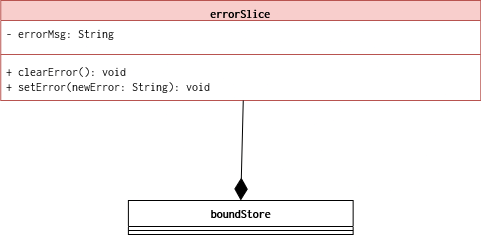
\includegraphics[width=0.7\textwidth]{images/UML/feature_model_errorSlice.drawio.png}
    \label{fig:UML_errorSlice}
    \caption{Diagramma UML dell'errorSlice}
\end{figure}
Questa slice contiene un eventuale messaggio di errore (\textbf{errorMsg}) e le corrispettive action per impostarlo o eliminarlo (\textbf{setError} e \textbf{clearError}). L'errore viene impostato da altre slice dello stato in caso di errori nell'aggiornamento dello stato. Le componenti, successivamente, controllano errorMsg per verificare se l'operazione richiesta è andata a buon fine.


\subsubsection{Componenti React}\label{sec:uml_react}
Per facilitare la lettura dei diagrammi delle componenti è stato scelto di organizzarli per feature in modo che ogni diagramma rappresenti le componenti che permettono di implementare aspetti chiave dell'applicazione.

I diagrammi prodotti che rappresentano funzionalità specifiche sono:
\begin{itemize}
    \item \textbf{Diagramma feature/setup} (\ref{fig:UML_feature_setup}): include le macro-componenti che costituiscono la pagina iniziale di configurazione del magazzino.
    \item \textbf{Diagramma feature/wmsLayout} (\ref{fig:UML_feature_wmsLayout}): include le macro-componenti di layout presenti nella pagina principale, i.e. le componenti che costituiscono header e sidebar.
    \item \textbf{Diagramma feature/actions} (\ref{fig:UML_feature_actions}): include tutte le macro-componenti che permettono all'utente di interagire con l'applicativo attraverso input testuali o pulsanti, nonché i dati informativi che si modificano in risposta alle azioni dell'utente sul magazzino.
    \item \textbf{Diagramma feature/render} (\ref{fig:UML_feature_render}): include tutte le macro-componenti che costituiscono gli elementi dell'ambiente 3D.
\end{itemize}


\paragraph{Feature/setup}
\begin{figure}[H]
    \centering
    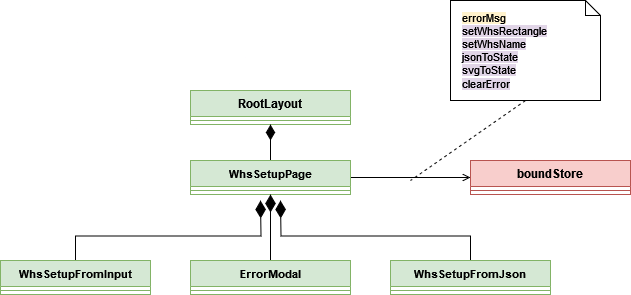
\includegraphics[width=0.8\textwidth]{images/UML/feature_setup.drawio.png}
    \label{fig:UML_feature_setup}
    \caption{Diagramma UML feature/setup}
\end{figure}

\subparagraph{\colorbox{verde_uml}{RootLayout}} \label{rootlayout}
\textbf{Tipo:} Presentational \\
\textbf{Interazioni con utente:} \\
Nessuna. \\
\textbf{Composizione}: \\
Contiene tutte le componenti di tutte le pagine dell'applicativo. \\
\textbf{Descrizione e funzionamento:} \\
Funge da contenitore principale per le informazioni di base e i tag HTML (\textit{\textless html\textgreater } e \textit{\textless body\textgreater }) utilizzati in tutte le pagine dell'applicazione. In altre parole, \textit{RootLayout }contiene i metadati e gli elementi HTML comuni a tutte le pagine, fornendo una struttura di base uniforme per l'intera applicazione. 

\subparagraph{\colorbox{verde_uml}{WhsSetupPage}}
\textbf{Tipo:} Container \\
\textbf{Accesso allo store:} \\
Chiama le action di configurare del magazzino (\textit{setWhsRectangle}, \textit{setWhsName}, \textit{svgToState} o \textit{jsonToState} a seconda dell'input fornito). Inoltre, rimane in ascolto per eventuali errori nell'esecuzione di tali operazioni, controllando il valore di \textit{errorMsg} nello store. Utilizza anche l'action \textit{clearError} per resettare l'errore e lasciare all'utente la possibilità di modificare quanto inserito con dati corretti.\\
\textbf{Composizione:} \\
\textit{WhsSetupPage} è costituita dalla componente \textit{Tabs} di Ant Design, dove ogni tab contiene uno dei moduli di configurazione del magazzino, i.e. \textit{WhsSetupFromInput} e \textit{WhsSetupFromJson}. Questo layout permette di visualizzare un solo form alla volta. Quando un form viene inviato, viene disabilitata l'altra tab. È inoltre presente una componente \textit{ErrorModal} per la visualizzazione di eventuali errori.\\
\textbf{Descrizione e funzionamento:} \\
Costituisce la pagina iniziale di configurazione del magazzino. Aggiorna lo stato del magazzino nello store con le informazioni ricevute da \textit{WhsSetupFromInput} o \textit{WhsSetupFromJson}. In caso di errori in tale aggiornamento, apre invece una finestra modale \textit{ErrorModal}.

\subparagraph{\colorbox{verde_uml}{WhsSetupFromInput}}
\textbf{Tipo:} Presentational \footnote[1]{\label{footnoteApi}Non accede allo store, tuttavia si occupa anche di una validazione preliminare di dati forniti da file esterni tramite il richiamo di un'API. Ques'API controlla che la struttura del file sia corretta, non occupandosi invece della correttezza dei dati stessi. Si è deciso di mantenere qui questa parte per minimizzare la complessità del componente padre \textit{WhsSetupPage}, mantenendo quest'ultimo più snello e focalizzato sulla gestione dello stato globale dell'applicazione e sul coordinamento delle diverse sue componenti figlie. Inoltre, chiamare l'API direttamente in questa componente consente di fornire un feedback più immediato all'utente tramite messaggi di errore (\textit{message.error} di Ant Design).} \\
\textbf{Interazione con l'utente:} \\
L'utente inserisce nome e dimensioni del magazzino nelle apposite caselle di input. Di default, le dimensioni includono altezza, larghezza e profondità, affinché sia possibile creare un magazzino quadrato/rettangolare. Tuttavia, gli utenti hanno anche la possibilità di caricare una planimetria personalizzata tramite un file SVG. Quando viene caricato tale file, le caselle di input per la larghezza e la profondità del magazzino vengono disabilitate. L'utente deve però inserire in ogni caso nome e altezza, poiché solo le dimensioni del pavimento del magazzino sono definite dalla planimetria caricata.  \\
\textbf{Composizione:} \\
Si tratta di una componente \textit{Form} di Ant Design che ha come \textit{Form.item} una componente \textit{Input} per il nome del magazzino, delle componenti \textit{InputNumber} per le dimensioni e una \textit{Upload} per il caricamento di un solo file SVG. \\
\textbf{Descrizione e funzionamento:} \\
Consente la configurazione del solo spazio del magazzino e dunque si utilizza nel caso in cui non si abbia ancora creato e salvato alcun magazzino.
L'utente compila il modulo seguendo le indicazioni fornite. Al momento poi dell'invio del modulo (se compilato correttamente e completamente), viene richiamata una funzione di \textit{WhsSetupPage} con i dati caricati e un valore indicante il caricamento o meno di planimetria personalizzata. Quest'ultimo segnala alla componente quale action (\textit{setWhsRectangle} o \textit{svgToState}) richiamare per la configurazione del pavimento del magazzino. 


\subparagraph{\colorbox{verde_uml}{WhsSetupFromJson}} 
\textbf{Tipo:} Presentational \textsuperscript{\ref{footnoteApi}} \\
\textbf{Interazione con l'utente:} \\
L'utente carica un file .json che include la configurazione del magazzino, i dati relativi agli elementi presenti al suo interno, nonché le richieste di movimentazione pendenti. \\
\textbf{Composizione:} \\
Si tratta di una componente \textit{Form} di Ant Design che ha come \textit{Form.item} una componente \textit{Upload} per il caricamento di un solo file JSON. \\
\textbf{Descrizione e funzionamento:} \\
Consente la configurazione dell'intero stato del magazzino e dunque si utilizza nel caso in cui si abbia già creato e salvato un magazzino in precedenza.
L'utente compila il modulo seguendo le indicazioni fornite. Al momento dell'invio del modulo (se compilato correttamente e completamente), viene richiamata una funzione di \textit{WhsSetupPage} con i dati caricati. Quest'ultima si occuperà di aggiornare lo stato tramite l'action \textit{jsonToState}.

\subparagraph{\colorbox{verde_uml}{ErrorModal}}\label{errorModal}
\textbf{Tipo:} Presentational \\
\textbf{Interazione con l'utente:} \\
L'utente può chiudere la finestra attraverso un apposito bottone.\\
\textbf{Composizione:} \\
È costituita dalla componente \textit{Modal} di Ant Design. \\
\textbf{Descrizione e funzionamento:} \\
Riceve il contenuto dello stato \textit{errorMsg} dalla componente Container padre e lo mostra come messaggio della finestra modale. Una volta chiusa la finestra viene richiamata una funzione della componente Container che si occupa di cancellare l'errore dallo stato (tramite \textit{clearError}) e riabilitare alla modifica la parte che ha causato l'errore.

\paragraph{Feature/wmsLayout}
\begin{figure}[H]
    \centering
    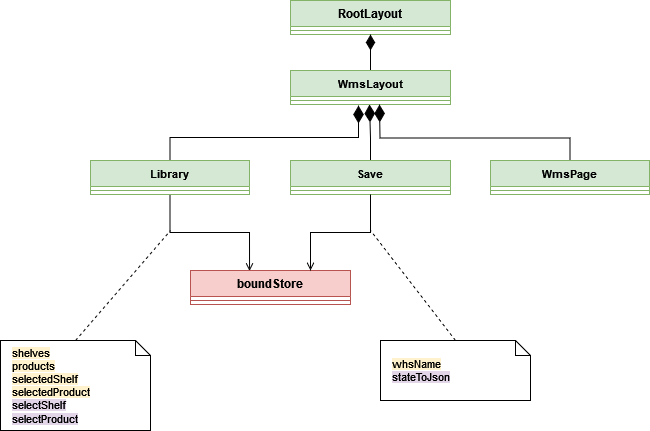
\includegraphics[width=0.9\textwidth]{images/UML/feature_wmsLayout.drawio.png}
    \label{fig:UML_feature_wmsLayout}
    \caption{Diagramma UML feature/wmsLayout}
\end{figure}

\subparagraph{\colorbox{verde_uml}{RootLayout}}
Si veda in \ref{rootlayout} per le specifiche.

\subparagraph{\colorbox{verde_uml}{WmsLayout}}
\textbf{Tipo:} Presentational \\
\textbf{Interazione con l'utente:} \\
L'utente può cliccare un bottone per aprire e chiudere la sidebar. \\
\textbf{Composizione:} \\
È costituito come componente \textit{Layout} di Ant Design, il quale a sua volta è costituito da \textit{Header}, \textit{Sider} e \textit{Content}.  La parte di \textit{Header} contiene un bottone di apertura e chiusura della sidebar, il logo e la componente \textit{Save}. La parte \textit{Sider}, i.e. la sidebar, contiene la componente \textit{Library}. Infine, la parte di \textit{Content} contiene la pagina principale \textit{WmsPage}.  \\
\textbf{Descrizione e funzionamento:} \\
Funge da contenitore secondario per la pagina principale dell'applicazione (\textit{WmsPage}) ed eventuali sue future pagine figlie. Si innesta infatti a RootLayout. 

\subparagraph{\colorbox{verde_uml}{Library}}
\textbf{Tipo:} Container \footnote[7]{In questo caso la parte Presentational è delegata alle componenti di Ant Design sue figlie.}\\
\textbf{Accesso allo store:} \\
\textit{Library} rimane in ascolto dello store per ottenere la lista aggiornata dei prodotti e scaffalature presenti nel magazzino (tramite gli stati \textit{products} e \textit{shelves}). \textit{Library} rimane anche in ascolto di \textit{selectedProduct} e \textit{selectedShelf} per avere sempre l'ultimo elemento selezionato e poterlo così evidenziare nell'elenco. Richiama inoltre \textit{selectProduct} o \textit{selectShelf} se l'utente clicca nella lista, rispettivamente, un prodotto o una scaffalatura. \\
\textbf{Composizione:} \\
È costituita principalmente da una componente \textit{Tree} di Ant Design che comprende la lista di tutte le scaffalature e prodotti presenti nel magazzino. Contiene inoltre una componente \textit{Search}, sempre di Ant Design, che consente di ricercare per nome un prodotto o scaffalatura in questa lista, filtrando l'albero stesso. \\
\textbf{Descrizione e funzionamento:} \\
Visualizza l'elenco di tutte le scaffalature e prodotti nel magazzino. L'utente può anche ricercare uno specifico elemento tramite nome attraverso la barra di ricerca fornita. Inoltre, se uno degli elementi della lista è selezionato, o tramite click o tramite selezione da render (quest'ultima solo per scaffalature, i prodotti in sé infatti non possono essere selezionati da render), questo viene evidenziato nella lista.

\subparagraph{\colorbox{verde_uml}{Save}}
\textbf{Tipo:} Container \footnote[7]{In questo caso la parte Presentational è delegata alle componenti di Ant Design sue figlie.}\\
\textbf{Accesso allo store:} \\
Se il bottone viene cliccato, viene chiamata l'action \textit{stateToJson}. \textit{Save} utilizza anche lo stato \textit{whsName} per denominare il file .json.\\
\textbf{Composizione:} \\
È costituita principalmente da una componente \textit{Button} di Ant Design. \\
\textbf{Descrizione e funzionamento:} \\
Viene utilizzato per salvare lo stato del magazzino in un file .json. Ricevuti i dati dallo store, viene creato un file .json con questi dati (denominato [\textit{whsName}].json). L'utente può dunque salvare in locale la configurazione attuale del magazzino, compresi tutti gli elementi al suo interno e le movimentazioni pendenti.

\subparagraph{\colorbox{verde_uml}{WmsPage}}\label{wmsPage}
\textbf{Tipo:} Presentational \\
\textbf{Interazione con l'utente:} \\
Nessuna.\\
\textbf{Composizione:} \\
Contiene il \textit{Render} e tutte le altre componenti con cui l'utente può interagire per apportare modifiche al magazzino o semplicemente visualizzarne lo stato. In particolare, contiene anche le componenti \textit{Tools}, \textit{ShelfManager}, \textit{ProductManager}, \textit{AllocationManager} e \textit{MovementManager}.\\
\textbf{Descrizione e funzionamento:} \\
Costituisce la pagina principale dell'applicazione. Il suo ruolo principale è infatti quello di contenitore e coordinatore della visibilità delle sue componenti figlie. Per far ciò utilizza gli hooks di React.\\

\begin{landscape}
\begin{figure}[H]
    \paragraph{Feature/actions}
    \centering
    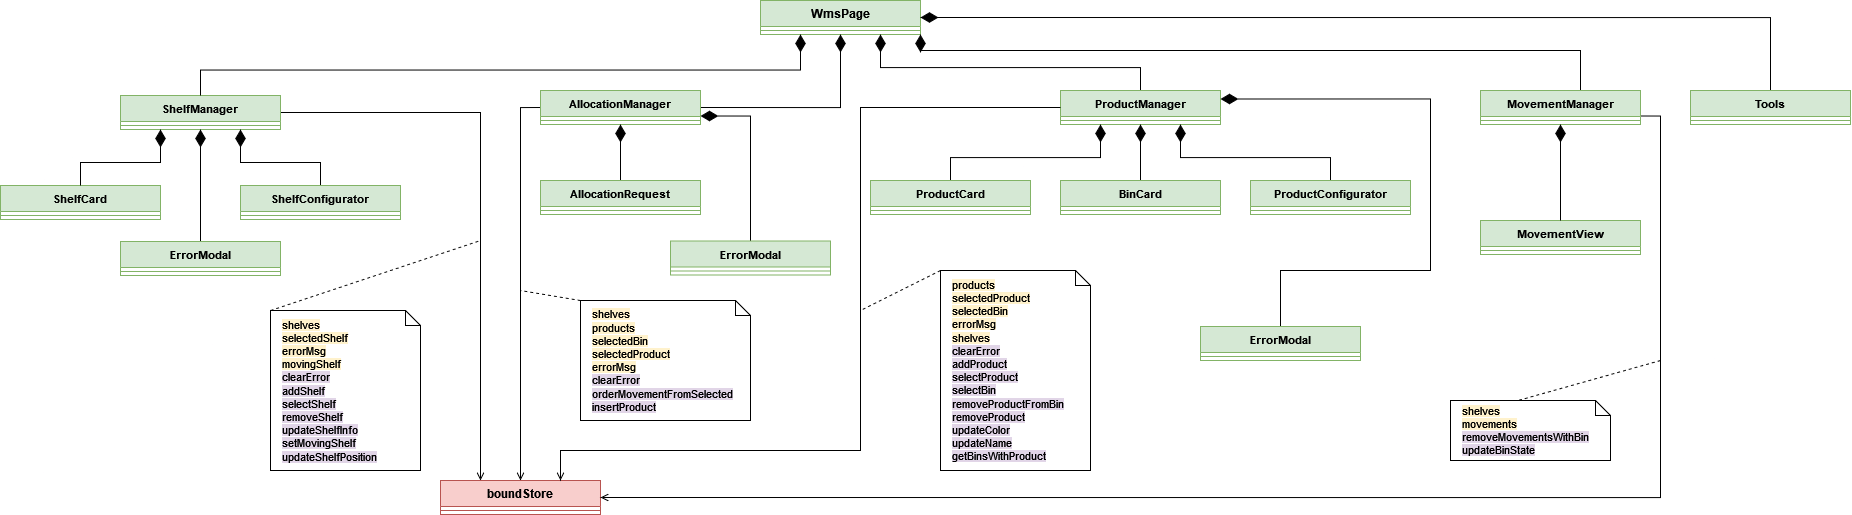
\includegraphics[width=1.5\textwidth]{images/UML/feature_actions.drawio.png}
    \label{fig:UML_feature_actions}
    \caption{Diagramma UML feature/actions}
\end{figure}
\end{landscape}
\newpage

\subparagraph{\colorbox{verde_uml}{WmsPage}}
Si veda in \ref{wmsPage} per le specifiche.

\subparagraph{\colorbox{verde_uml}{ShelfManager}}
\textbf{Tipo:} Container \\
\textbf{Accesso allo store:} \\
Accede allo store per avere lo stato aggiornato di tutte le scaffalature (\textit{shelves}) e/o per modificarlo in risposta alle azioni compiute dall'utente attraverso le componenti figlie (a seconda dell'azione attraverso \textit{addShelf}, \textit{removeShelf}, \textit{updateShelfInfo} o \textit{updateShelfPosition}). Oltre a ciò, utilizza \textit{selectedShelf}, \textit{movingShelf}, \textit{selectShelf} e \textit{setMovingShelf} per coordinare le operazioni con il render. Utilizza \textit{selectedShelf} anche per aprire la \textit{ShelfCard} corrispondente. Inoltre, rimane in ascolto per eventuali errori nell'esecuzione di tali operazioni, controllando il valore di \textit{errorMsg} nello store. Utilizza anche l'action \textit{clearError} per resettare l'errore e lasciare all'utente la possibilità di modificare quanto inserito con dati corretti.
\\
\textbf{Composizione:} \\
Contiene le componenti \textit{ShelfCard} per la visualizzazione dei dati di una scaffalatura, \textit{ShelfConfigurator} per l'aggiunta/modifica di una scaffalatura e \textit{ErrorModal} per la visualizzazione di eventuali errori.
\\
\textbf{Descrizione e funzionamento:} \\
È responsabile della gestione delle scaffalature nel magazzino, inclusa l'aggiunta, la modifica e la semplice visualizzazione dei dati a essa relativi. 
Nello specifico, se è presente una scaffalatura selezionata (\textit{selectedShelf}) ne ricava le informazioni e li visualizza tramite la componente figlia \textit{ShelfCard}. Altrimenti, se riceve indicazione da \textit{WmsPage} o dalla \textit{ShelfCard} stessa, apre \textit{ShelfConfigurator} rispettivamente per l'aggiunta o per la modifica di una scaffalatura.  Inoltre, se viene segnalata l'eliminazione di una scaffalatura da parte di \textit{ShelfCard}, \textit{ShelfManager} provvede alla sua rimozione.
In caso di errori nell'aggiornamento dello stato, apre anche una componente \textit{ErrorModal}.

\subparagraph{\colorbox{verde_uml}{ShelfConfigurator}}
\textbf{Tipo:} Presentational \\
\textbf{Interazione con l'utente:} \\
In caso di aggiunta di una scaffalatura, l'utente inserisce nome e dimensioni della scaffalature nelle apposite caselle di input. In caso di modifica, si limita a modificare le parti desiderate. Si procede poi con l'eventuale modifica della posizione da render.\\
\textbf{Composizione:} \\
È costituito da un componente \textit{Drawer} di Ant Design, contenente a sua volta un componente \textit{Steps}, sempre di Ant Design. Quest'ultimo divide il processo di creazione/modifica in due parti: una prima parte dedicata al nome e alle misure, disponibile tramite una componente \textit{Form}, e una seconda parte per il posizionamento. Quest'ultimo può avvenire solamente tramite render quindi qui viene riportata solo una semplice descrizione di come eseguirlo. Per quanto riguarda il \textit{Form}, invece, questo contiene i \textit{Form.item} per il nome (tipo \textit{Input}), per la dimensione del bin (tipo \textit{InputNumber}), per la capacità in altezza (tipo \textit{InputNumber}) e larghezza (tipo \textit{InputNumber}). Sono presenti anche alcuni pulsanti per chiudere il \textit{Drawer} annullando le modifiche oppure per procedere con il step successivo/confermare le modifiche.\\
\textbf{Descrizione e funzionamento:} \\
Viene utilizzato per aggiungere una scaffalatura al magazzino o modificarne una già presente. In questo secondo caso, il \textit{Form} fornito è già completato con i dati correnti della scaffalatura selezionata (\textit{selectedShelf)}. L'utente compila/modifica il modulo seguendo le indicazioni date. Al momento poi dell'invio del modulo (se compilato correttamente e completamente), viene richiamata una funzione di \textit{ShelfManager} con i dati caricati. Quest'ultima controlla attraverso un hook di React, precedentemente impostato, se i dati inviati riguardano una scaffalatura esistente e procede a richiamare l'action dello store corrispondente (\textit{addShelf} o \textit{updateShelfInfo}). Alla conferma finale della creazione, dopo il posizionamento da render, \textit{ShelfConfigurator} richiama un'altra funzione di \textit{ShelfManager} che aggiorna la posizione della scaffalatura nello store (tramite \textit{updateShelfPosition}).

\newpage
\subparagraph{\colorbox{verde_uml}{ShelfCard}}
\textbf{Tipo:} Presentational \\
\textbf{Interazione con l'utente:} \\
L'utente può cliccare dei pulsanti per modificare oppure per eliminare la scaffalatura.\\
\textbf{Composizione:} \\
È costituita da una componente \textit{Card} di Ant Design, il cui titolo è dato dal nome della scaffalatura e la descrizione ne tutte contiene le dimensioni. Inoltre, contiene due pulsanti utilizzati per eliminare la scaffalatura oppure modificarla.\\
\textbf{Descrizione e funzionamento:} \\
Viene utilizzata principalmente per visualizzare i dati relativi alla scaffalatura correntemente selezionata. Quest'ultimi sono ricevuti come props da \textit{ShelfManager}. L'utente può anche decidere di eliminare o modificare la scaffalatura tramite alcuni pulsanti. Questi richiamano delle funzioni di \textit{ShelfManager} che aggiornano lo stato con l'eliminazione della scaffalatura nel primo caso (tramite \textit{removeShelf}) e aprono \textit{ShelfConfigurator} per la modifica nel secondo. 

\subparagraph{\colorbox{verde_uml}{ProductManager}}
\textbf{Tipo:} Container \\
\textbf{Accesso allo store:} \\
Accede allo store per avere lo stato aggiornato di tutti i prodotti (\textit{products}) e bin (attraverso \textit{shelves}) e/o per modificarlo in risposta alle azioni compiute dall'utente attraverso le componenti figlie (a seconda dell'azione attraverso \textit{addProduct}, \textit{removeProduct}, \textit{updateName}, \textit{updateColor} o \textit{removeProductFromBin}). Oltre a ciò, utilizza \textit{selectedProduct}, \textit{selectedBin}, \textit{selectProduct} e \textit{selectBin} per coordinare la visualizzazione e le operazioni tra le sue componenti figlie. Inoltre, utilizza \textit{getBinsWithProduct} per ottenere una lista di tutti i bin in cui il prodotto è presente. Infine, rimane in ascolto per eventuali errori nell'esecuzione delle operazioni sopra-elencate, controllando il valore di \textit{errorMsg} nello store. Utilizza anche l'action \textit{clearError} per resettare l'errore e lasciare all'utente la possibilità di modificare quanto inserito con dati corretti.
\\
\textbf{Composizione:} \\
Contiene le componenti \textit{ProductCard} per la visualizzazione dei dati generali del prodotto, \textit{BinCard} per la visualizzazione dei dati del prodotto in un specifico bin, \textit{ProductConfigurator} per l'aggiunta/modifica di un prodotto e \textit{ErrorModal} per la visualizzazione di eventuali errori.
\\
\textbf{Descrizione e funzionamento:} \\
È responsabile della gestione dei prodotti nel magazzino, inclusa l'aggiunta, la modifica e la semplice visualizzazione dei dati a esso relativi. 
Nello specifico, se è presente un bin selezionato (\textit{selectedBin}) ne ricava le informazioni e le visualizza tramite \textit{BinCard}. Analogamente, se è presente un prodotto selezionato (\textit{selectedProduct}), ne ricava le informazioni e le visualizza tramite la componente figlia \textit{ProductCard}. Altrimenti, se riceve indicazione da \textit{WmsPage} o dalla \textit{ProductCard} stessa, apre \textit{ShelfConfigurator} rispettivamente per l'aggiunta o per la modifica di un prodotto.  Inoltre, se viene segnalata l'eliminazione di un prodotto da parte di \textit{ProductCard} o da \textit{BinCard}, \textit{ProductManager} provvede alla sua rimozione (rispettivamente tramite \textit{removeProduct}, che rimuove completamente il prodotto dal magazzino, e \textit{removeProductFromBin}, che lo rimuove solamente dal bin selezionato). Alla stessa maniera, se viene segnalato il posizionamento di un prodotto da parte di \textit{ProductCard} o \textit{BinCard}, \textit{ProductManager} provvede a tale operazione segnalando a \textit{WmsPage} la volontà di aprire l'\textit{AllocationManager} (nel primo caso per posizionamento di un prodotto e nel secondo per una richiesta di movimentazione).
In caso di errori nell'aggiornamento dello stato, apre anche una componente \textit{ErrorModal}.

\subparagraph{\colorbox{verde_uml}{ProductConfigurator}}
\textbf{Tipo:} Presentational \\
\textbf{Interazione con l'utente:} \\
In caso di aggiunta di un prodotto, l'utente inserisce nome e sceglie il colore del prodotto negli appositi spazi di input. In caso di modifica, si limita a modificare le parti desiderate. \\
\textbf{Composizione:} \\
È costituito da un componente \textit{Drawer} di Ant Design, contenente a sua volta una componente \textit{Form}, Quest'ultimo 
contiene i \textit{Form.item} per il nome (tipo \textit{Input}), 
e per il colore (tipo \textit{ColorPicker}). Sono presenti anche due pulsanti per chiudere il \textit{Drawer} annullando le modifiche oppure per confermare la creazione.\\
\textbf{Descrizione e funzionamento:} \\
Viene utilizzato per aggiungere un prodotto al magazzino o modificarne uno già presente. In questo secondo caso, il \textit{Form} fornito è già completato con i dati correnti del prodotto selezionato (\textit{selectedProduct}). L'utente compila/modifica il modulo seguendo le indicazioni date. Al momento poi dell'invio del modulo (se compilato correttamente e completamente), viene richiamata una funzione di \textit{ProductManager} con i dati caricati. Quest'ultima controlla attraverso un hook di React, precedentemente impostato, se i dati inviati riguardano un prodotto esistente e procede a richiamare l'action dello store corrispondente (\textit{addProduct} oppure \textit{updateName}+\textit{updateColor}).

\subparagraph{\colorbox{verde_uml}{ProductCard}}
\textbf{Tipo:} Presentational \\
\textbf{Interazione con l'utente:} \\
L'utente può cliccare dei pulsanti per modificare, per eliminare oppure per posizionare un prodotto.\\
\textbf{Composizione:} \\
È costituita da una componente \textit{Card} di Ant Design, il cui titolo è dato dal nome del prodotto e la descrizione ne contiene il colore e una componente \textit{Table} di Ant Design con la lista di tutti i bin in cui il prodotto è allocato. Inoltre, contiene tre pulsanti utilizzati per eliminare, modificare e allocare il prodotto.\\
\textbf{Descrizione e funzionamento:} \\
Viene utilizzata principalmente per visualizzare i dati relativi al prodotto correntemente selezionato nella sua interezza. Questi dati sono ricevuti come props da \textit{ProductManager}.  L'utente può anche decidere di eliminare, modificare oppure allocare un prodotto tramite alcuni pulsanti. Questi richiamano delle funzioni di \textit{ProductManager} che aggiornano lo stato con l'eliminazione della scaffalatura nel primo caso (tramite \textit{removeProduct}), aprono \textit{ProductConfigurator} per la modifica nel secondo oppure segnalano ad \textit{AllocationManager} la volontà di allocare un prodotto nel terzo. Inoltre, se l'utente clicca su uno specifico bin in cui è allocato il prodotto nella \textit{Table} della \textit{ProductCard}, sarà possibile selezionare tale bin tramite \textit{ProductManager} e aprire dunque la \textit{BinCard} a esso relativa.

\subparagraph{\colorbox{verde_uml}{BinCard}}
\textbf{Tipo:} Presentational \\
\textbf{Interazione con l'utente:} \\
L'utente può cliccare dei pulsanti per eliminare il prodotto presente nel bin oppure per richiederne lo spostamento.\\
\textbf{Composizione:} \\
È costituita da una componente \textit{Card} di Ant Design, il cui titolo è dato dall'id del bin e la descrizione ne tutte contiene lo stato e il prodotto inserito (se presente). Inoltre, contiene due pulsanti utilizzati per eliminare il prodotto contenuto (se presente) oppure per richiederne lo spostamento (sempre se è presente un prodotto).\\
\textbf{Descrizione e funzionamento:} \\
Viene utilizzata principalmente per visualizzare i dati relativi ad un prodotto specifico correntemente selezionato (\textit{selectedBin}). Quest'ultimi sono ricevuti come props da \textit{ProductManager}. L'utente può anche decidere di eliminare o richiederne lo spostamento tramite alcuni pulsanti. Questi richiamano delle funzioni di \textit{ProductManager} che aggiornano lo stato con l'eliminazione del prodotto dal bin nel primo caso (tramite \textit{removeProductFromBin}) e segnalano ad \textit{AllocationManager} la volontà di movimentare un prodotto nel secondo. Nel caso in cui il bin sia vuoto questi pulsanti richiamano un \textit{message.error} di Ant Design che informa l'utente dell'impossibilità di eseguire tali operazioni.

\subparagraph{\colorbox{verde_uml}{AllocationManager}}
\textbf{Tipo:} Container \\
\textbf{Accesso allo store:} \\
Accede allo store per avere lo stato aggiornato di tutte le scaffalature (\textit{shelves}) e prodotti (\textit{products}), necessario per poter fornire tutti i dati ad \textit{AllocationRequest}. Accede allo store anche per modificare lo stato in risposta alle azioni compiute dall'utente attraverso \textit{AllocationRequest} (a seconda dell'azione attraverso \textit{orderMovementFromSelected} o \textit{insertProduct}). Oltre a ciò, rimane in ascolto di \textit{selectedBin} e \textit{selectedProduct} per poter aprire l'\textit{AllocationRequest} correttamente.
Infine, rimane in ascolto anche per eventuali errori nell'esecuzione di tali operazioni, controllando il valore di \textit{errorMsg} nello store. Utilizza anche l'action \textit{clearError} per resettare l'errore e lasciare all'utente la possibilità di modificare quanto inserito con dati corretti.\\
\textbf{Composizione:} \\
Contiene le componenti \textit{AllocationRequest} e \textit{ErrorModal} per la visualizzazione di eventuali errori.\\
\textbf{Descrizione e funzionamento:} \\
È responsabile della gestione del posizionamento dei prodotti nelle scaffalature, sia per quanto riguarda l'allocazione sia per la richiesta di movimentazione. 
Nello specifico, se riceve indicazione da \textit{WmsPage} ed è presente un prodotto selezionato (\textit{selectedProduct}) o un bin selezionato (\textit{selectedBin}) apre \textit{AllocationRequest}. \textit{AllocationRequest} sarà dunque dedicato all'allocazione se a essere selezionato è il prodotto in sé, mentre sarà dedicato alla movimentazione se a essere selezionato è il bin. Si occupa poi di aggiornare lo stato con i dati ricevuti da \textit{AllocationRequest}.
In caso di errori durante tale aggiornamento, \textit{AllocationManager} apre anche una componente \textit{ErrorModal}.

\subparagraph{\colorbox{verde_uml}{AllocationRequest}}
\textbf{Tipo:} Presentational \\
\textbf{Interazione con l'utente:} \\
L'utente seleziona la posizione (scaffalatura e ripiano+colonna della scaffalatura stessa) in cui inserire il prodotto. \\
\textbf{Composizione:} \\
È costituito da un componente \textit{Drawer} di Ant Design, contenente a sua volta una componente \textit{Form}, Quest'ultimo 
contiene i \textit{Form.item} per la scaffalatura di destinazione (selezionabile tramite \textit{Select}), per il ripiano della scaffalatura di destinazione (selezionabile tramite \textit{Select}) e per la colonna della scaffalatura di destinazione (selezionabile tramite \textit{Select}). Sono presenti anche due pulsanti per chiudere il \textit{Drawer} annullando le modifiche oppure per confermare il posizionamento.\\
\textbf{Descrizione e funzionamento:} \\
Viene utilizzato per allocare un prodotto nel magazzino o per richiedere la movimentazione di uno già allocato. In questo secondo caso, il \textit{Form} fornito contiene anche l'indicazione del bin di origine (\textit{selectedBin}). L'utente compila/modifica il modulo seguendo le indicazioni date. Al momento poi dell'invio del modulo (se compilato correttamente e completamente), viene richiamata una funzione di \textit{AllocationManager} con i dati caricati. Quest'ultima controlla attraverso un hook di React, precedentemente impostato, se i dati inviati riguardano un prodotto già allocato e procede a richiamare l'action dello store corrispondente (\textit{orderMovementFromSelected} o \textit{insertProduct}).

\subparagraph{\colorbox{verde_uml}{MovementManager}}
\textbf{Tipo:} Container \\
\textbf{Accesso allo store:} \\
Accede allo store per avere lo stato aggiornato di tutte le scaffalature (\textit{shelves}) e movimentazioni pendenti (\textit{movements}), necessario per poter fornire tutti i dati a \textit{MovementView}. Accede allo store anche per modificare lo stato in risposta alle azioni compiute dall'utente attraverso \textit{MovementView} (attraverso \textit{removeMovementsWithBin} e \textit{updateBinState}).\\
\textbf{Composizione:} \\
È composto dalla componente \textit{MovementView}.\\
\textbf{Descrizione e funzionamento:} \\
È responsabile della gestione delle richieste di movimento pendenti. 
Nello specifico, se riceve indicazione da \textit{WmsPage} apre \textit{MovementView}. Attraverso \textit{MovementView} sarà possibile vedere le richieste pendenti e, per ciascuna, richiedere un sollecito. Il sollecito viene effettuato sotto forma di chiamata API ad un meccanismo esterno che ritorna ``True'' se la movimentazione è stata accettata o ``False'' se rifiutata. In base a questo valore \textit{MovementManager} aggiornerà lo stato tramite \textit{updateBinState} e \textit{removeMovementsWithBin}.

\newpage
\subparagraph{\colorbox{verde_uml}{MovementView}}
\textbf{Tipo:} Presentational \\
\textbf{Interazione con l'utente:} \\
L'utente può cliccare dei pulsanti di sollecito, presenti per ciascuna richiesta di movimentazione pendente.\\
\textbf{Composizione:} \\
È costituito da un componente \textit{Drawer} di Ant Design, contenente a sua volta una componente \textit{List}. Ogni \textit{List.item} ha come descrizione scaffalatura e bin di origine e destinazione della movimentazione e come action un pulsante di sollecito della movimentazione.\\
\textbf{Descrizione e funzionamento:} \\
Viene utilizzato principalmente per visualizzare tutte le movimentazioni ancora pendenti e richiederne il disbrigo tramite apposito pulsante. Quest'ultima funzionalità è resa possibile tramite chiamata di una funzione di \textit{MovementManager}. 

\subparagraph{\colorbox{verde_uml}{Tools}}
\textbf{Tipo:} Presentational \\
\textbf{Interazione con l'utente:} \\
L'utente può cliccare dei pulsanti per aggiungere nuovi prodotti o scaffalature e visualizzare/sollecitare le richieste di movimentazione di prodotti.
\\
\textbf{Composizione:} \\
È costituita principalmente da componenti \textit{FloatButton} di Ant Design, accompagnate da \textit{ToolTip} che ne chiariscono l'utilizzo. In particolare, include un singolo \textit{FloatButton} impiegato per aprire la lista delle movimentazioni pendenti, e un \textit{FloatButton.Group} che contiene i pulsanti \textit{FloatButton} utilizzati per aggiungere elementi (scaffalature e prodotti) al magazzino.\\
\textbf{Descrizione e funzionamento:} \\
Funge da piattaforma centralizzata per l'accesso a varie funzionalità legate al magazzino, tra cui l'aggiunta di scaffalature e prodotti, nonché la gestione delle movimentazioni pendenti.
Se cliccati i bottoni di aggiunta scaffalatura o prodotto vengono visualizzati i form di configurazione presenti in \textit{ShelfManager} e \textit{ProductManager}. Se invece viene cliccato il pulsante di apertura della lista dei movimenti viene visualizzato tramite \textit{MovementManager} un elenco di tutte le richieste pendenti. L'apertura di tutte queste componenti è gestita attraverso il passaggio dello stato dei click di questi pulsanti a \textit{WmsPage}. Come accennato, quest'ultima si occuperà poi di aprire le giuste componenti figlie tramite hooks di React. 

\subparagraph{\colorbox{verde_uml}{ErrorModal}}
Si veda in \ref{errorModal} per le specifiche.


\paragraph{Feature/render}
\begin{figure}[H]
    \centering
    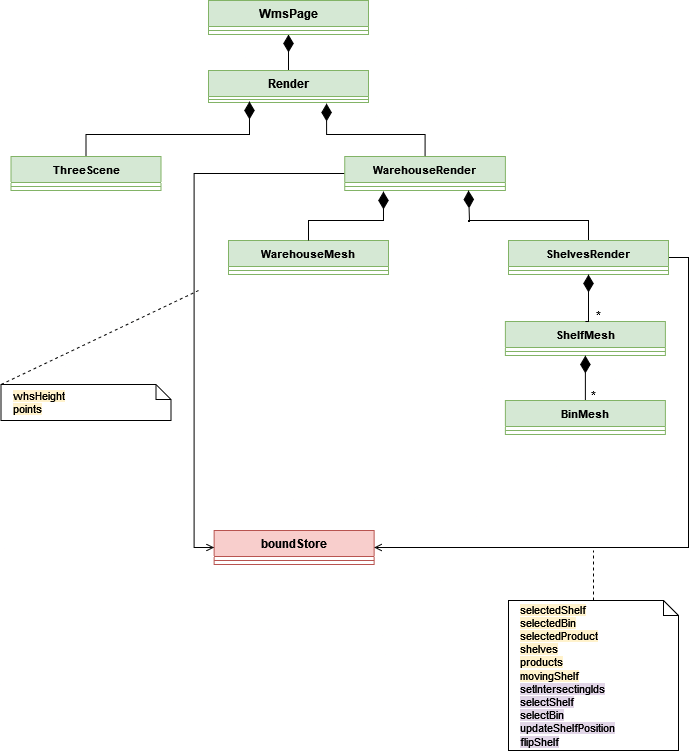
\includegraphics[width=0.9\textwidth]{images/UML/feature_render.drawio.png}
    \label{fig:UML_feature_render}
    \caption{Diagramma UML feature/render}
\end{figure}

\subparagraph{\colorbox{verde_uml}{WmsPage}}
Si veda in \ref{wmsPage} per le specifiche.

\subparagraph{\colorbox{verde_uml}{Render}}
\textbf{Tipo:} Presentational \\
\textbf{Interazione con l'utente:} \\
L'utente può abilitare il cambiamento della vista tramite click del tasto centrale del mouse. \\
\textbf{Composizione:} \\
È costituita da una componente \textit{KeyboardControls} di react-three/drei e una \textit{Canvas} di react-three/drei. Quest'ultima contiene, a sua volta, le componenti \textit{ThreeScene} e \textit{WarehouseRender}.\\
\textbf{Descrizione e funzionamento:} \\
Serve principalmente come contenitore della vista 3D del magazzino. Tuttavia, viene utilizzata anche per coordinare l'utilizzo della tastiera tra gli usi esterni al render 3D e quelli interni, i.e. di cambiamento della vista. In particolare, viene utilizzato un hook di React, passato come prop a \textit{ThreeScene}, per abilitare o meno questa proprietà. \\

\subparagraph{\colorbox{verde_uml}{ThreeScene}}
\textbf{Tipo:} Presentational \\
\textbf{Interazione con l'utente:} \\
L'utente può utilizzare il mouse o la tastiera per cambiare la vista del magazzino 3D.\\ 
\textbf{Composizione:} \\
È composta dalle componenti \textit{CameraControls}, \textit{ambientLight} e \textit{gridHelper}.\\
\textbf{Descrizione e funzionamento:} \\
Serve a configurare la scena di Three.js. In particolare, aggiunge una luce e una griglia utile a dare delle coordinate all'utente per quanto riguarda la pavimentazione del magazzino. Sono presenti anche dei controlli per la camera per consentire il cambiamento della vista da tastiera e da mouse.\\

\subparagraph{\colorbox{verde_uml}{WarehouseRender}}
\textbf{Tipo:} Container \\
\textbf{Accesso allo store:} \\
Accede allo store per \textit{whsHeight} e \textit{points} per fornire i dati del magazzino a \textit{WarehouseMesh}.\\
\textbf{Composizione:} \\
È composta dalle componenti \textit{ShelvesRender} e \textit{WarehouseMesh}.\\
\textbf{Descrizione e funzionamento:} \\
Serve da coordinatore tra le mesh delle scaffalature presenti nel magazzino (create da \textit{ShelvesRender}) e la mesh del magazzino stesso (\textit{WarehouseMesh}). In particolare, memorizza i riferimenti di queste mesh.

\subparagraph{\colorbox{verde_uml}{WarehouseMesh}}
\textbf{Tipo:} Presentational \\
\textbf{Interazione con l'utente:} \\
Nessuna.\\
\textbf{Composizione:} \\
Si tratta di una componente \textit{group}, che raccoglie in sé delle componenti \textit{Extrude} di react-three/drei per il pavimento e per ciascun muro. \\
\textbf{Descrizione e funzionamento:} \\
Serve alla costruzione della mesh del magazzino. Per ogni coppia di punti in \textit{points}, ricevuti dalla componente \textit{WarehouseRender}, viene creata una linea che viene estrusa con profondità \textit{whsHeight}, misura anch'essa ricevuta come prop da \textit{WarehouseRender}. Sempre attraverso \textit{points}, viene creata una \textit{Shape} di Three.js per il pavimento del magazzino.

\subparagraph{\colorbox{verde_uml}{ShelvesRender}}
\textbf{Tipo:} Container \\
\textbf{Accesso allo store:} \\
Accede allo store per avere lo stato aggiornato di tutte le scaffalature (\textit{shelves}), necessario per poter visualizzare in 3D le scaffalature aggiornate all'ultima modifica. Rimane in ascolto anche per \textit{selectedProduct}, \textit{selectedBin} e \textit{selectedShelf} per poter evidenziare nel render l'elemento selezionato. Nel caso la selezione avvenga da render, si utilizza \textit{selectBin} e \textit{selectShelf} per aggiornare lo stato. Utilizza inoltre \textit{movingShelf} se è presenta una scaffalatura in movimentazione. In quest'ultimo caso, inoltre, accede allo store anche per modificare lo stato in risposta alla movimentazione (attraverso \textit{updateShelfPosition}, \textit{flipShelf} e \textit{setIntersectingIds}).\\
\textbf{Composizione:} \\
Contiene una \textit{ShelfMesh} per ogni scaffalatura presente in \textit{shelves}. Contiene inoltre delle componenti \textit{TransformControls} di react-three/drei attivati per la movimentazione e rotazione delle scaffalature in movimento (\textit{movingShelf}).\\
\textbf{Descrizione e funzionamento:} \\
Si occupa della gestione delle mesh delle scaffalature. 
In particolare, si occupa di aggiornare lo store quando scaffalature o bin vengono selezionati dal render (attraverso rispettivamente \textit{selectShelf} e \textit{selectBin}). Si occupa anche di controllare le collisioni tra scaffalature e mesh del magazzino e, di conseguenza, aggiornare la posizione nello store (attraverso \textit{updateShelfPosition}). Inoltre, si occupa anche della movimentazione stessa delle scaffalature in movimento (\textit{movingShelf}) attraverso i \textit{TransformControls}.

\subparagraph{\colorbox{verde_uml}{ShelfMesh}}
\textbf{Tipo:} Presentational \\
\textbf{Interazione con l'utente:} \\
Nessuna.\\
\textbf{Composizione:} \\
Si tratta di un \textit{group}, che raccoglie in sé componenti \textit{BinMesh} per ogni bin della scaffalatura.\\
\textbf{Descrizione e funzionamento:} \\
Serve alla costruzione della mesh di una scaffalatura. Vengono create delle \textit{BinMesh} per ogni bin della scaffalatura passata come prop. Queste vengono poi posizionati in modo tale da avere una matrice di mesh [\textit{height} della scaffalatura][\textit{width} della scaffalatura] con posizione centrale dell'intera matrice uguale alla posizione della scaffalatura passata come prop. 

\subparagraph{\colorbox{verde_uml}{BinMesh}}
\textbf{Tipo:} Presentational \\
\textbf{Interazione con l'utente:} \\
L'utente può selezionare la scaffalatura cliccando sulla \textit{BinMesh}. Se la scaffalatura è già selezionata, si seleziona il bin invece. Se invece è il bin a essere già selezionato, si seleziona la scaffalatura.\\
\textbf{Composizione:} \\
È composta da una \textit{mesh} con geometria \textit{boxGeometry} rappresentante il bin e un'altra interna più piccola rappresentare il prodotto contenuto, se esistente. È presente anche una componente \textit{Edges} di react-three/drei utilizzata in caso di selezione di un bin o di un prodotto.\\
\textbf{Descrizione e funzionamento:} \\
Costruisce fisicamente in 3D il bin e l'eventuale prodotto contenuto. Il bin viene rappresentato come un cubo di dimensione fornita da \textit{ShelfMesh} (dato dalla \textit{binSize} memorizzata nello store per tale scaffalatura). Sono poi applicati diversi materiali ai lati di questo cubo per farlo somigliare ad una scaffalatura. Viene anche utilizzata una texture per segnalare colonna e ripiano dei bin. Per quanto riguarda il prodotto, anche questo viene rappresentato come un cubo del colore fornito da \textit{ShelfMesh} (dato dal colore memorizzato nello store per tale prodotto). In caso di stati particolari del bin, vengono applicate delle texture al prodotto per segnalare ciò. Sia per prodotto che per bin, infine, in caso di selezione viene modificato il colore del bin e/o utilizzata una componente \textit{Edges} per il prodotto.

\subsubsection{API}
Questa sezione fornisce una panoramica delle varie API implementate nel progetto, delineandone lo scopo, le funzionalità e l'utilizzo. Si precisa l'utilizzo dell'\textbf{API routes} di Next.js per l'implementazione di tali API. Questa soluzione permette di instradare e gestire le richieste dei client in modo efficiente, consentendo un'interazione fluida e affidabile con il server, oltre che facilitare lo sviluppo, il debug e il testing.

\paragraph{jsonParser}
\textbf{Scopo:}\\
Si occupa della validazione iniziale dei dati JSON. In particolare, verifica che i dati JSON ricevuti siano conformi alla struttura e al formato richiesti dall'applicazione.

\bigskip
\noindent \textbf{Funzionalità:}\\
L'API richiama una funzione \textit{isValidJson(jsonData)} che prende un oggetto JSON come input ed esegue vari controlli per validarne la struttura. Verifica la presenza di chiavi essenziali come \textit{products}, \textit{shelves}, \textit{whsName}, \textit{whsHeight}, \textit{whsPoints} e \textit{movements}. Inoltre, garantisce che queste chiavi contengano i tipi e i formati di dati previsti:
\begin{itemize}
    \item Per \textit{products}, ogni prodotto nei dati JSON deve avere una proprietà \textit{id} (tipo stringa), \textit{name} (tipo stringa) e \textit{color} (tipo oggetto).
    \item Per \textit{shelves}: ogni scaffalatura deve avere una proprietà \textit{id} (tipo stringa), \textit{name} (tipo stringa), \textit{binSize} (tipo numero), \textit{width} (tipo numero), \textit{height} (tipo numero), \textit{isFlipped} (tipo boolean) e \textit{bins} (tipo array di oggetti bin).
    \item Per \textit{bins}: ogni oggetto bin deve avere una proprietà \textit{id} (tipo stringa), \textit{state} (tipo stringa) e una proprietà facoltativa \textit{productId} (tipo stringa oppure null).
\end{itemize}
La funzione restituisce ``True'' se i dati JSON sono validi secondo i criteri sopra specificati; in caso contrario, restituisce ``False''.

\noindent Dopo aver ricevuto indicazione da questa funzione, l'API genera dunque risposte JSON contenenti messaggi di stato e di errore in base al risultato ottenuto.

\bigskip
\noindent \textbf{Utilizzo nel progetto:}\\
Questa API viene utilizzata da \textit{WhsSetupFromJson} per gestire richieste POST contenenti file JSON. Dopo la ricezione dei dati, l'API li sottopone a una serie di controlli per convalidarli prima che siano elaborati ulteriormente. In particolare, questo test serve ad assicurarsi che il formato e struttura del file sia quello generato dal salvataggio del magazzino tramite l'applicazione. Se la convalida dei dati fallisce, al client viene restituita una risposta di errore appropriata. Si noti che non si controlla la validità dei dati stessi, che sarà invece controllata al momento dell'inserimento nello store. Tuttavia, questo approccio impedisce l'accesso a quest'ultimo per l'aggiornamento con dati sicuramente errati o incompleti.

\paragraph{svgParser}
\textbf{Scopo:}\\
Si occupa della validazione iniziale dei file SVG. Essa verifica la presenza di elementi specifici all'interno del file SVG per garantirne la conformità alle richieste dell'applicazione.

\bigskip
\noindent \textbf{Funzionalità:}\\
L'API richiama una funzione \textit{isValidSVG(svgData)} che utilizza la libreria JSDOM per analizzare e manipolare il contenuto SVG ricevuto. In particolare, questa funzione crea un documento DOM virtuale, estrae gli elementi SVG pertinenti e applica le regole di validazione per determinare la conformità del file SVG. In particolare, gli elementi SVG che controlla sono:
\begin{itemize}
    \item La presenza di elementi \textit{polygon};
    \item La presenza di almeno uno di questi con proprietà \textit{points} definita.
\end{itemize}
Dunque, se almeno un poligono contiene punti, il file SVG viene considerato valido e viene restituito ``True''. Altrimenti, viene ritornato ``False''.

\noindent Dopo aver ricevuto indicazione da questa funzione, l'API genera dunque risposte JSON contenenti messaggi di stato e di errore in base al risultato ottenuto.

\bigskip
\noindent \textbf{Utilizzo nel progetto:}\\
Questa API viene utilizzata da \textit{WhsSetupFromInput} per gestire richieste POST contenenti file SVG. Dopo la ricezione dei dati, l'API li sottopone a una serie di controlli per convalidarli prima che siano elaborati ulteriormente. In particolare, questo test serve ad assicurarsi che il formato e struttura del file renda possibile la creazione di un pavimento personalizzato a forma poligonale. Se la convalida dei dati fallisce, al client viene restituita una risposta di errore appropriata. Si noti che non si controlla la validità dei dati stessi, che sarà invece controllata al momento dell'inserimento nello store. Tuttavia, questo approccio impedisce l'accesso a quest'ultimo per l'aggiornamento con dati sicuramente errati o incompleti.

\paragraph{movementRequest}
\textbf{Scopo:}\\
Questa API è progettata per ricevere richieste relative ai movimenti all'interno dell'applicazione e determinare se devono essere accettate o rifiutate. Il suo scopo principale è emulare il processo di decisione automatizzato per le richieste di movimento.

\bigskip
\noindent \textbf{Funzionalità:}\\
L'API accetta richieste contenenti l'identificatore del movimento (\textit{movementId}) e utilizza un algoritmo di simulazione per determinare lo stato della richiesta (accettata o rifiutata) in base a una probabilità casuale generata. L'API genera poi risposte JSON contenenti il messaggio relativo allo stato della richiesta.

\bigskip
\noindent \textbf{Utilizzo nel progetto:}\\
Questa API viene utilizzata da \textit{movementManager} per il disbrigo delle richieste di movimento di prodotti all'interno del magazzino. Va notato che l'implementazione di questa API non è inclusa nel capitolato, bensì è sviluppata internamente dal proponente. Pertanto, questa API viene attualmente impiegata esclusivamente a fini di simulazione. Infatti, il suo utilizzo serve unicamente a fornire una rappresentazione pratica del processo decisionale automatico nel contesto operativo.

%%%%%%%%%%%%%%%%%%%%%%%%%%%%%%%%%%%
% ARCHITETTURA DI DEPLOYMENT
%%%%%%%%%%%%%%%%%%%%%%%%%%%%%%%%%%%
\section{Architettura di deployment}\label{sec:architettura_deployment}
Il gruppo ha deciso di adottare una architettura \textit{Serverless} per il deployment. 
Essa consente agli sviluppatori di creare e gestire applicazioni senza doversi preoccupare dell'infrastruttura sottostante. Infatti, con ``serverless'' non si intende l'assenza totale di server, bensì l'assenza di questi e della loro gestione nell'esperienza di sviluppo. Infatti, tutte le attività di gestione dei server ricadono su un fornitore di servizi cloud.

In particolare, il gruppo ha deciso di utilizzare \textbf{Vercel} come piattaforma di hosting che supporta questo tipo di architettura. La scelta di questo strumento rispetto ad altri con le stesse funzionalità è dettata dalla sua alta integrazione con Next.js (utilizzato anch'esso nello sviluppo del progetto).
\bigskip

\noindent Un'architettura \textit{Serverless} porta a vantaggi quali:
\begin{itemize}
    \item \textbf{Automazione:} le soluzioni serverless eliminano infatti la fatica di gestire i server automatizzando le attività;
    \item \textbf{Scalabilità:} le soluzioni serverless aumentano e diminuiscono automaticamente in risposta al traffico senza la necessità di ottimizzazioni o altre configurazioni manuali;
    \item \textbf{Produttività:} le soluzioni serverless consentono agli sviluppatori di concentrarsi sulla scrittura del codice e sull'ottimizzazione dello stesso anziché dedicare tempo alla gestione dei server;
    \item \textbf{Semplicità di gestione:} e.g. con Vercel, è sufficiente collegare la cartella GitHub al servizio ed ogni volta che vengono apportate modifiche al repository GitHub, l'applicazione viene automaticamente rilasciata e aggiornata sulla piattaforma di hosting senza ulteriori interventi manuali.
\end{itemize}


%%%%%%%%%%%%%%%%%%%%%%%%%%%%%%%%%%%
% REQUISITI
%%%%%%%%%%%%%%%%%%%%%%%%%%%%%%%%%%%
\section{Stato dei requisiti funzionali}\label{sec:requisiti}
Di seguito vengono riportati i requisiti funzionali corredati dal loro stato: ``Soddisfatto'' o ``Non soddisfatto''.
Per una visione più completa sui requisiti si rimanda al documento \textit{Analisi dei Requisiti v5.0.0}.

\rowcolors{2}{gray!10!}{white}
\renewcommand{\arraystretch}{2.5}
\begin{xltabular}{\textwidth}{ p{0.1\textwidth} | X | p{0.3\textwidth} }
    \rowcolor{black}
    \textbf{\color{white} Codice} & \textbf{\color{white} Descrizione} & \textbf{\color{white} Stato} \\ 
    \endhead

    \caption{Stato dei requisiti funzionali} 
    \endlastfoot

    ROF\_1 & L'utente può creare un ambiente di magazzino tridimensionale & Soddisfatto\\
    ROF\_1.1 & L'utente può creare un ambiente di magazzino tridimensionale da zero & Soddisfatto\\
    ROF\_1.1.1 & L'utente può creare una planimetria personalizzata & Soddisfatto\\
    RDF\_1.2 & L'utente può caricare un layout memorizzato in database per inizializzare l'ambiente & Non soddisfatto\\
    RFF\_1.3 & L'utente può caricare un file in formato svg per inizializzare l'ambiente & Soddisfatto \\
    RDF\_2 & L'utente può salvare i dati del magazzino creato in un database & Non soddisfatto\\  
    RDF\_2.1 & L'utente salva i dati dello spazio del magazzino & Soddisfatto \\ 
    RDF\_2.2 & L'utente salva i dati delle scaffalature presenti nel magazzino & Soddisfatto \\  
    RDF\_2.3 & L'utente salva i dati dei prodotti presenti del magazzino & Soddisfatto \\    
    ROF\_3 & L'utente può visualizzare tutto il magazzino in 3D & Soddisfatto\\
    ROF\_3.1 & L'utente può visualizzare lo spazio del magazzino in 3D & Soddisfatto\\
    ROF\_3.2 & L'utente può visualizzare le scaffalature posizionate all'interno del magazzino in 3D & Soddisfatto\\
    ROF\_3.3 & L'utente può visualizzare i prodotti posizionati all'interno del magazzino in 3D & Soddisfatto\\
    RFF\_3.3.1 & L'utente può visualizzare i prodotti creati (non posizionati) in 3D & Non soddisfatto \\      
    ROF\_4 & L'utente può navigare attraverso lo spazio tridimensionale & Soddisfatto\\
    ROF\_4.1 & L'utente deve poter ingrandire l'area di visione a cui è interessato & Soddisfatto \\
    ROF\_4.2 & L'utente deve poter rimpicciolire l'area di visione a cui è interessato & Soddisfatto \\
    ROF\_4.3 & L'utente deve poter ruotare orizzontalmente la camera & Soddisfatto \\
    ROF\_4.4 & L'utente deve poter ruotare verticalmente la camera & Soddisfatto \\
    ROF\_4.5 & L'utente può navigare nello spazio tridimensionale attraverso il mouse& Soddisfatto\\
    ROF\_4.6 & L'utente può navigare nello spazio tridimensionale attraverso la tastiera& Soddisfatto\\
    ROF\_5 & L'utente può visualizzare in un'area gestionale separata (la libreria) l'elenco degli oggetti creati & Soddisfatto \\
    ROF\_5.1 & L'utente può visualizzare l'elenco delle scaffalature create & Soddisfatto\\
    ROF\_5.1.1 & L'utente per ogni scaffalatura deve poterne visualizzare il codice & Soddisfatto\\
    ROF\_5.1.2 & L'utente per ogni scaffalatura deve poterne visualizzare le dimensioni & Soddisfatto\\
    ROF\_5.1.3 & L'utente per ogni scaffalatura deve poterne visualizzare le dimensioni dei bin & Soddisfatto\\
    ROF\_5.2 & L'utente può visualizzare l'elenco dei prodotti creati & Soddisfatto \\
    ROF\_5.2.1 & L'utente per ogni prodotto deve poterne visualizzare il nome & Soddisfatto\\
    %ROF\_5.2.2 & L'utente per ogni prodotto deve poterne visualizzare le dimensioni & Implicito, Discussione interna [UC4.2.1.2]\\
    ROF\_5.2.2 & L'utente per ogni prodotto posizionato all'interno del magazzino deve poterne visualizzare la posizione & Soddisfatto \\
    ROF\_6 & L'utente può creare delle scaffalature & Soddisfatto\\
    ROF\_6.1 & L'utente può scegliere un codice univoco da dare alla scaffalatura & Soddisfatto\\
    ROF\_6.2 & L'utente può scegliere la dimensione delle scaffalature & Soddisfatto\\
    ROF\_6.2.1 & Le scaffalature devono essere divise in bin codificabili con coordinate & Soddisfatto\\
    ROF\_6.2.2 & L'utente può scegliere la dimensione del bin per la scaffalatura & Soddisfatto\\
    ROF\_7 & L'utente può inserire le scaffalature nello spazio 3D & Soddisfatto\\
    ROF\_8 & L'utente può selezionare una scaffalatura & Soddisfatto\\
    ROF\_8.1 & L'utente può selezionare una scaffalatura dalla libreria & Soddisfatto\\
    RFF\_8.1.1 & La scaffalatura è evidenziata in libreria quando viene selezionata & Soddisfatto\\
    ROF\_8.2 & L'utente può selezionare una scaffalatura dal render 3D & Soddisfatto\\
    RFF\_8.2.1 & La scaffalatura è evidenziata nel render 3D quando viene selezionata & Soddisfatto\\
    ROF\_9 & L'utente può modificare una scaffalatura creata & Soddisfatto\\
    ROF\_9.1 & L'utente può modificare la capacità della scaffalatura & Soddisfatto\\
    RDF\_9.2 & L'utente può modificare il codice della scaffalatura & Soddisfatto\\
    RDF\_9.3 & L'utente può modificare la posizione della scaffalatura & Soddisfatto\\
    RDF\_10 & L'utente può ricercare per codice una scaffalatura & Soddisfatto\\
    ROF\_11 & L'utente può eliminare una scaffalatura creata & Soddisfatto\\
    ROF\_11.1 & L'utente può cancellare la scaffalatura dalla libreria & Soddisfatto\\
    ROF\_11.2 & L'utente può cancellare la scaffalatura dal render 3D & Soddisfatto\\
    ROF\_12 & L'utente può creare un prodotto di forma parallelepipeda & Soddisfatto\\
    ROF\_12.1 & L'utente può scegliere un nome univoco da dare al prodotto & Soddisfatto\\
    %RDF\_12.2 & L'utente può scegliere delle dimensioni da dare al prodotto & Esplicito, Verbale esterno 04-12-23 [UC13.2]\\  
    ROF\_13 & L'utente può inserire i prodotti in un bin di una scaffalatura all'interno dello spazio 3D & Soddisfatto\\
    ROF\_14 & L'utente può selezionare un prodotto creato & Soddisfatto\\
    ROF\_14.1 & L'utente può selezionare un prodotto dalla libreria & Soddisfatto\\
    RFF\_14.1.1 & Il prodotto è evidenziato in libreria quando viene selezionato & Soddisfatto\\
    ROF\_14.2 & L'utente può selezionare un prodotto posizionato dal render 3D & Soddisfatto\\
    RFF\_14.2.1 & Il prodotto è evidenziato nel render 3D quando viene selezionato & Soddisfatto\\
    RDF\_15 & L'utente può ricercare per nome un prodotto & Soddisfatto\\
    ROF\_16 & L'utente può eliminare un prodotto creato & Soddisfatto\\
    ROF\_16.1 & L'utente può eliminare un prodotto creato dalla libreria & Soddisfatto\\
    ROF\_16.2 & L'utente può eliminare un prodotto posizionato dal render 3D & Soddisfatto\\
    ROF\_17 & L'utente può richiedere lo spostamento di un oggetto & Soddisfatto\\
    RDF\_17.1 & L'utente può richiedere lo spostamento tramite trascinamento & Non soddisfatto\\
    ROF\_17.2 & L'utente può richiedere lo spostamento tramite click del mouse & Soddisfatto\\
    ROF\_18 & Il sistema deve verificare la disponibilità della scaffalatura target alla richiesta di uno spostamento & Soddisfatto\\
    ROF\_19 & Il sistema delega ad un meccanismo terzo la decisione finale sull'accettazione di un movimento & Soddisfatto\\
    RFF\_20 & L'utente può codificare il magazzino in aree specifiche per uno scopo & Non soddisfatto\\
    \hline
\end{xltabular}

\subsection{Grafici riassuntivi di copertura}
\begin{figure}[H]
    \centering
    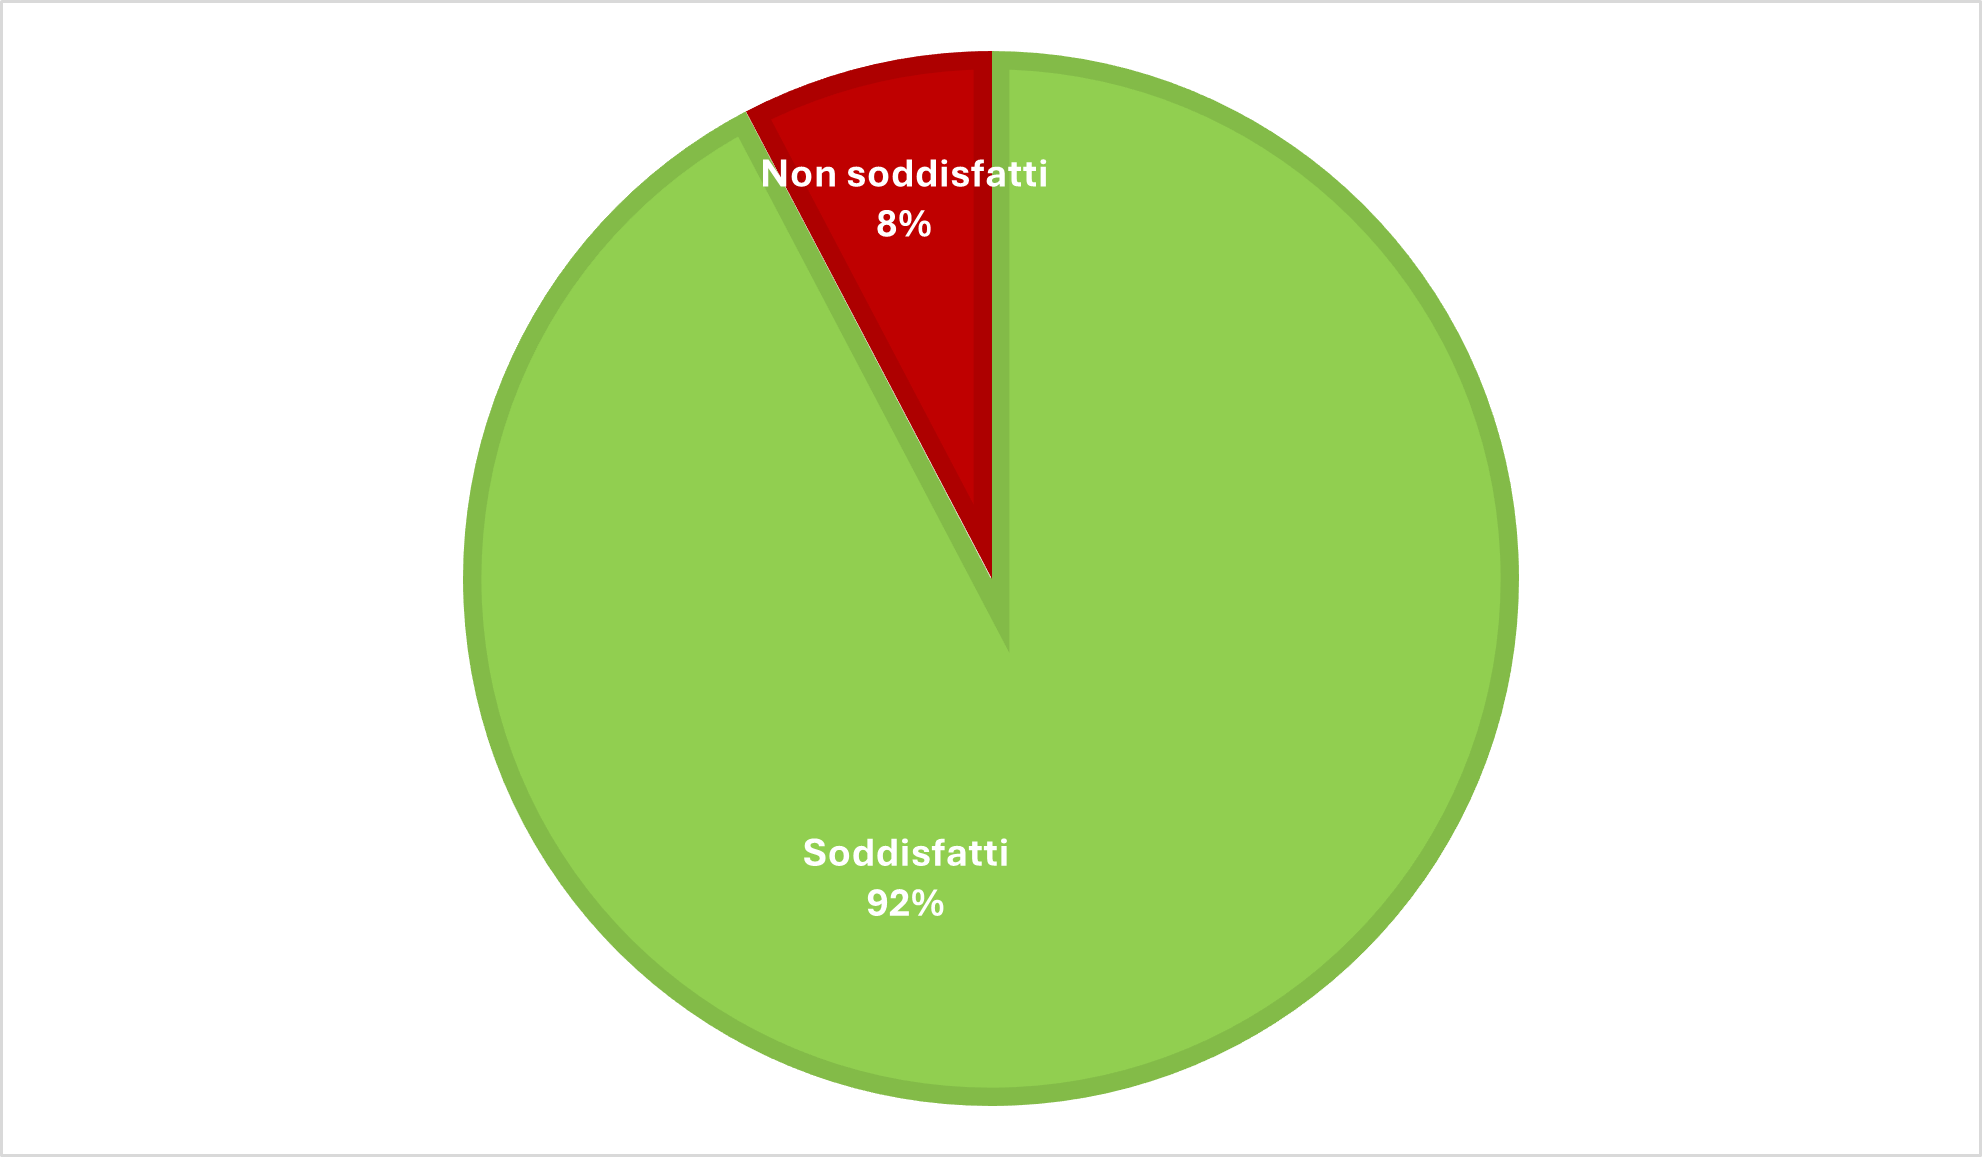
\includegraphics[width=0.7\textwidth]{images/stato_req_totali.png}
    \caption{Grafico dello stato di copertura dei requisiti totali}
\end{figure}

\begin{figure}[H]
    \centering
    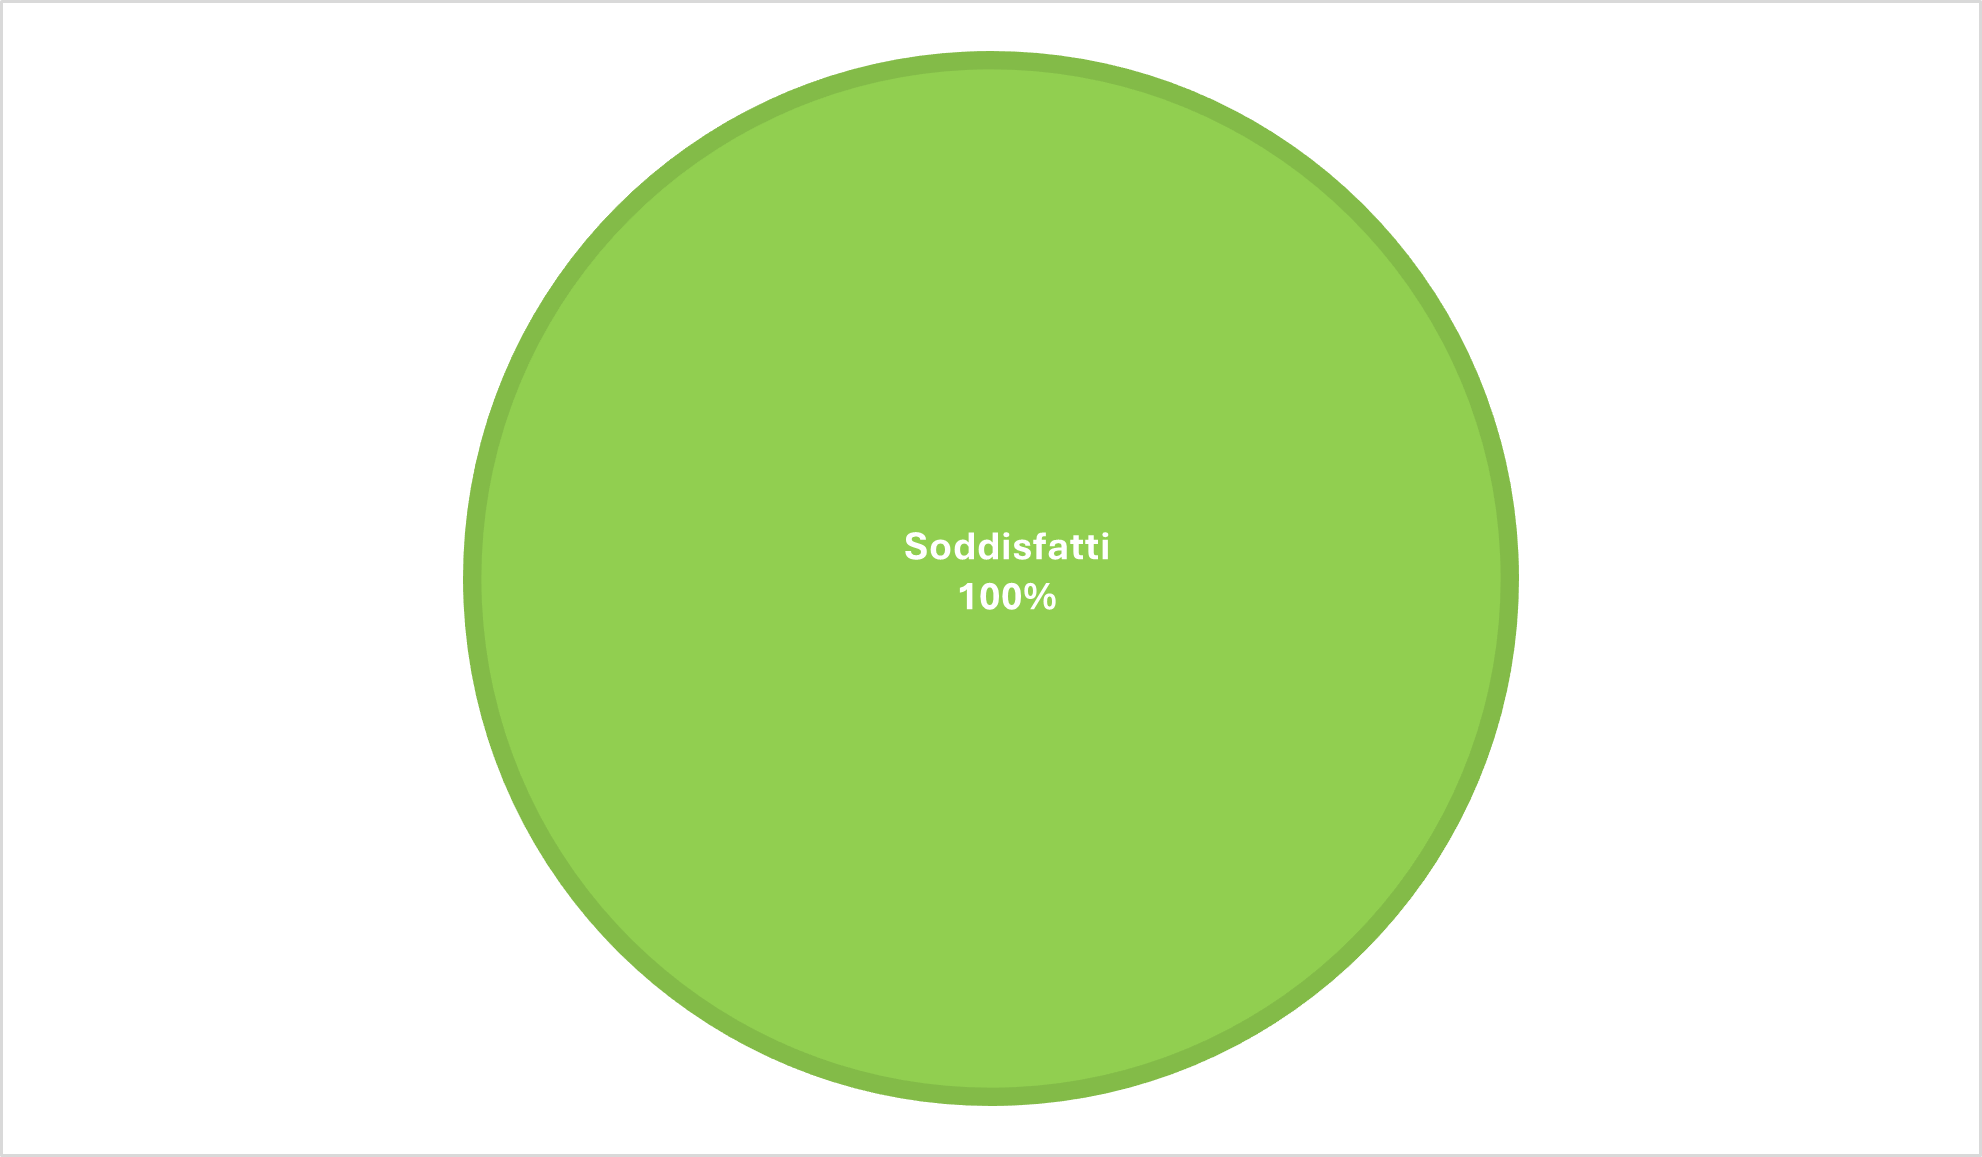
\includegraphics[width=0.7\textwidth]{images/stato_req_obbligatori.png}
    \caption{Grafico dello stato di copertura dei requisiti funzionali obbligatori}
\end{figure}

\begin{figure}[H]
    \centering
    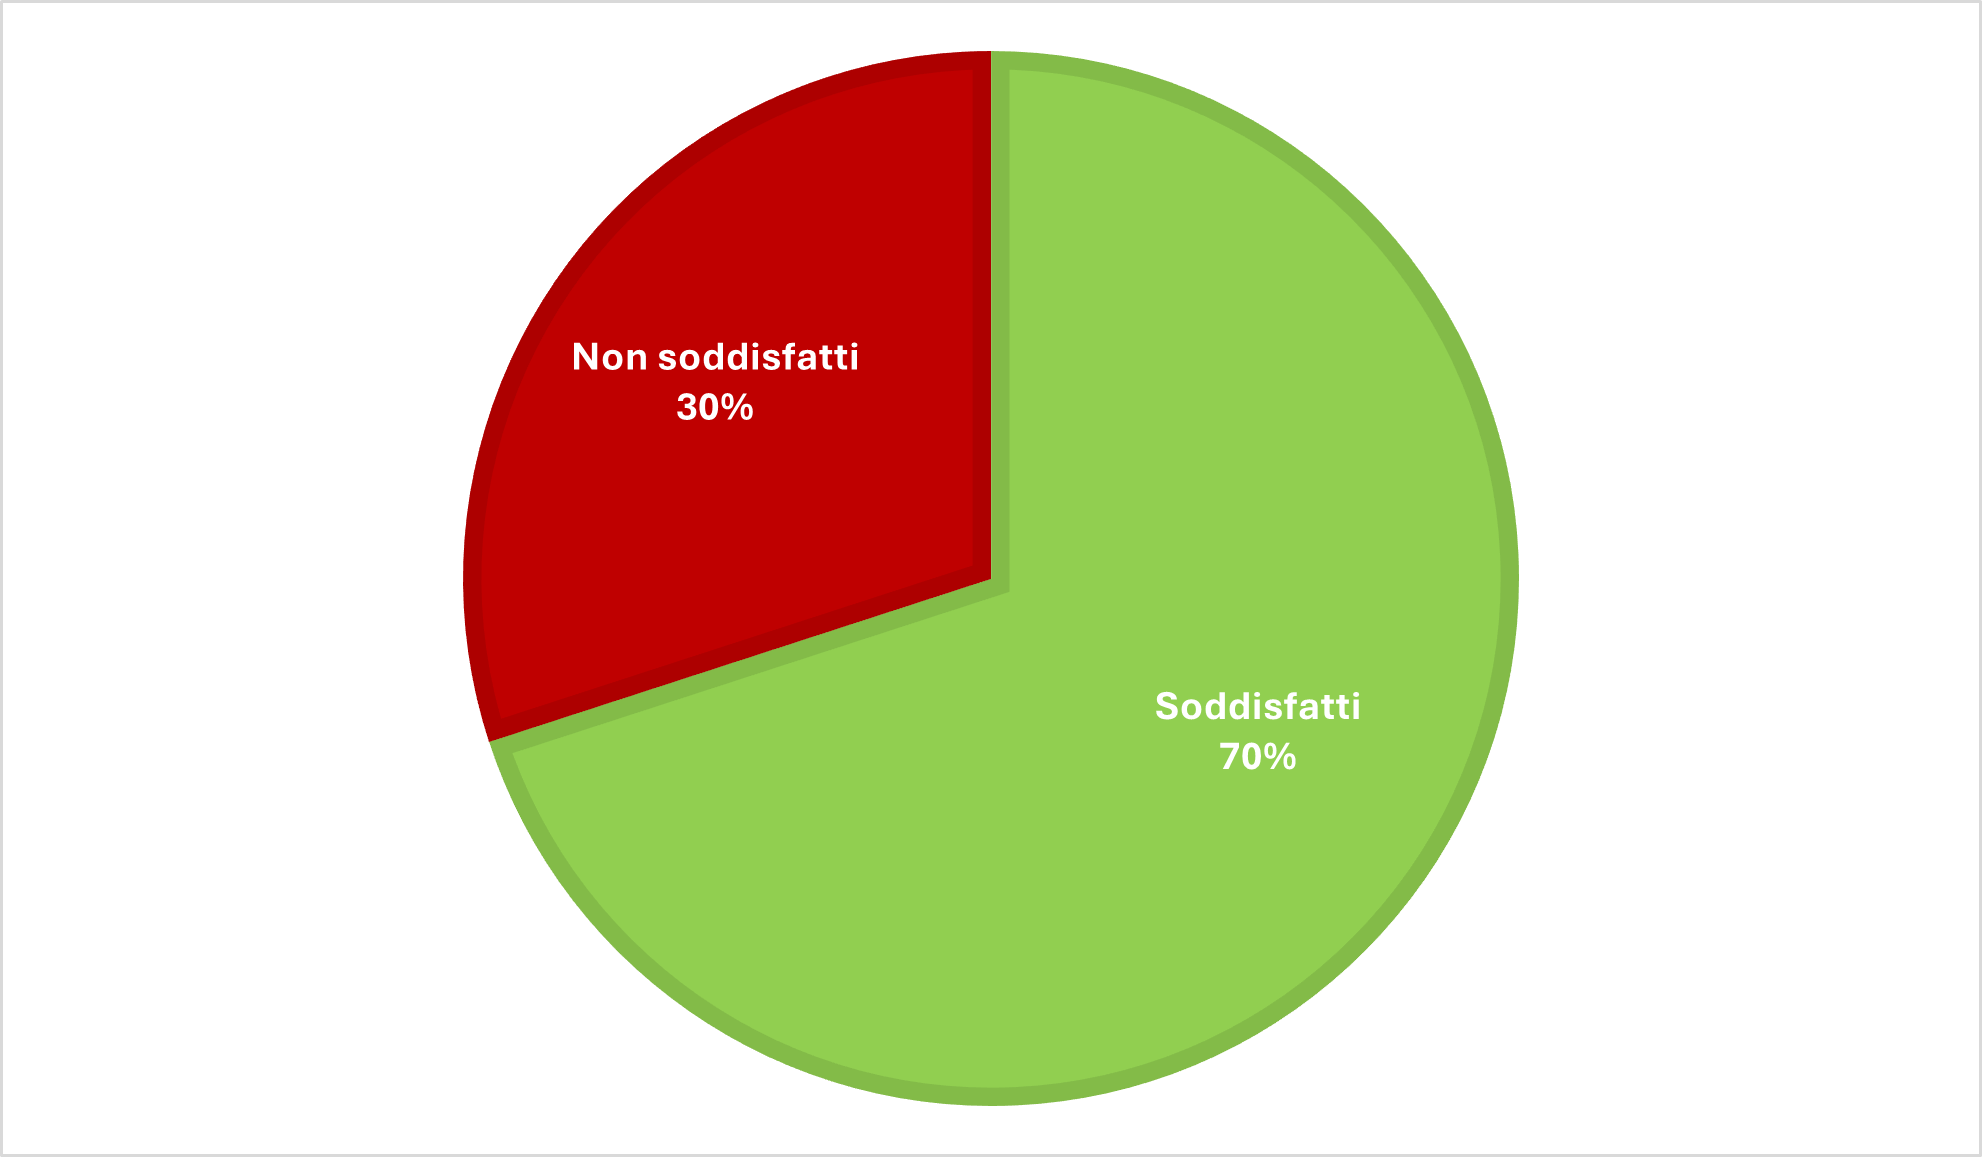
\includegraphics[width=0.7\textwidth]{images/stato_req_desiderabili.png}
    \caption{Grafico dello stato di copertura dei requisiti funzionali desiderabili}
\end{figure}

\begin{figure}[H]
    \centering
    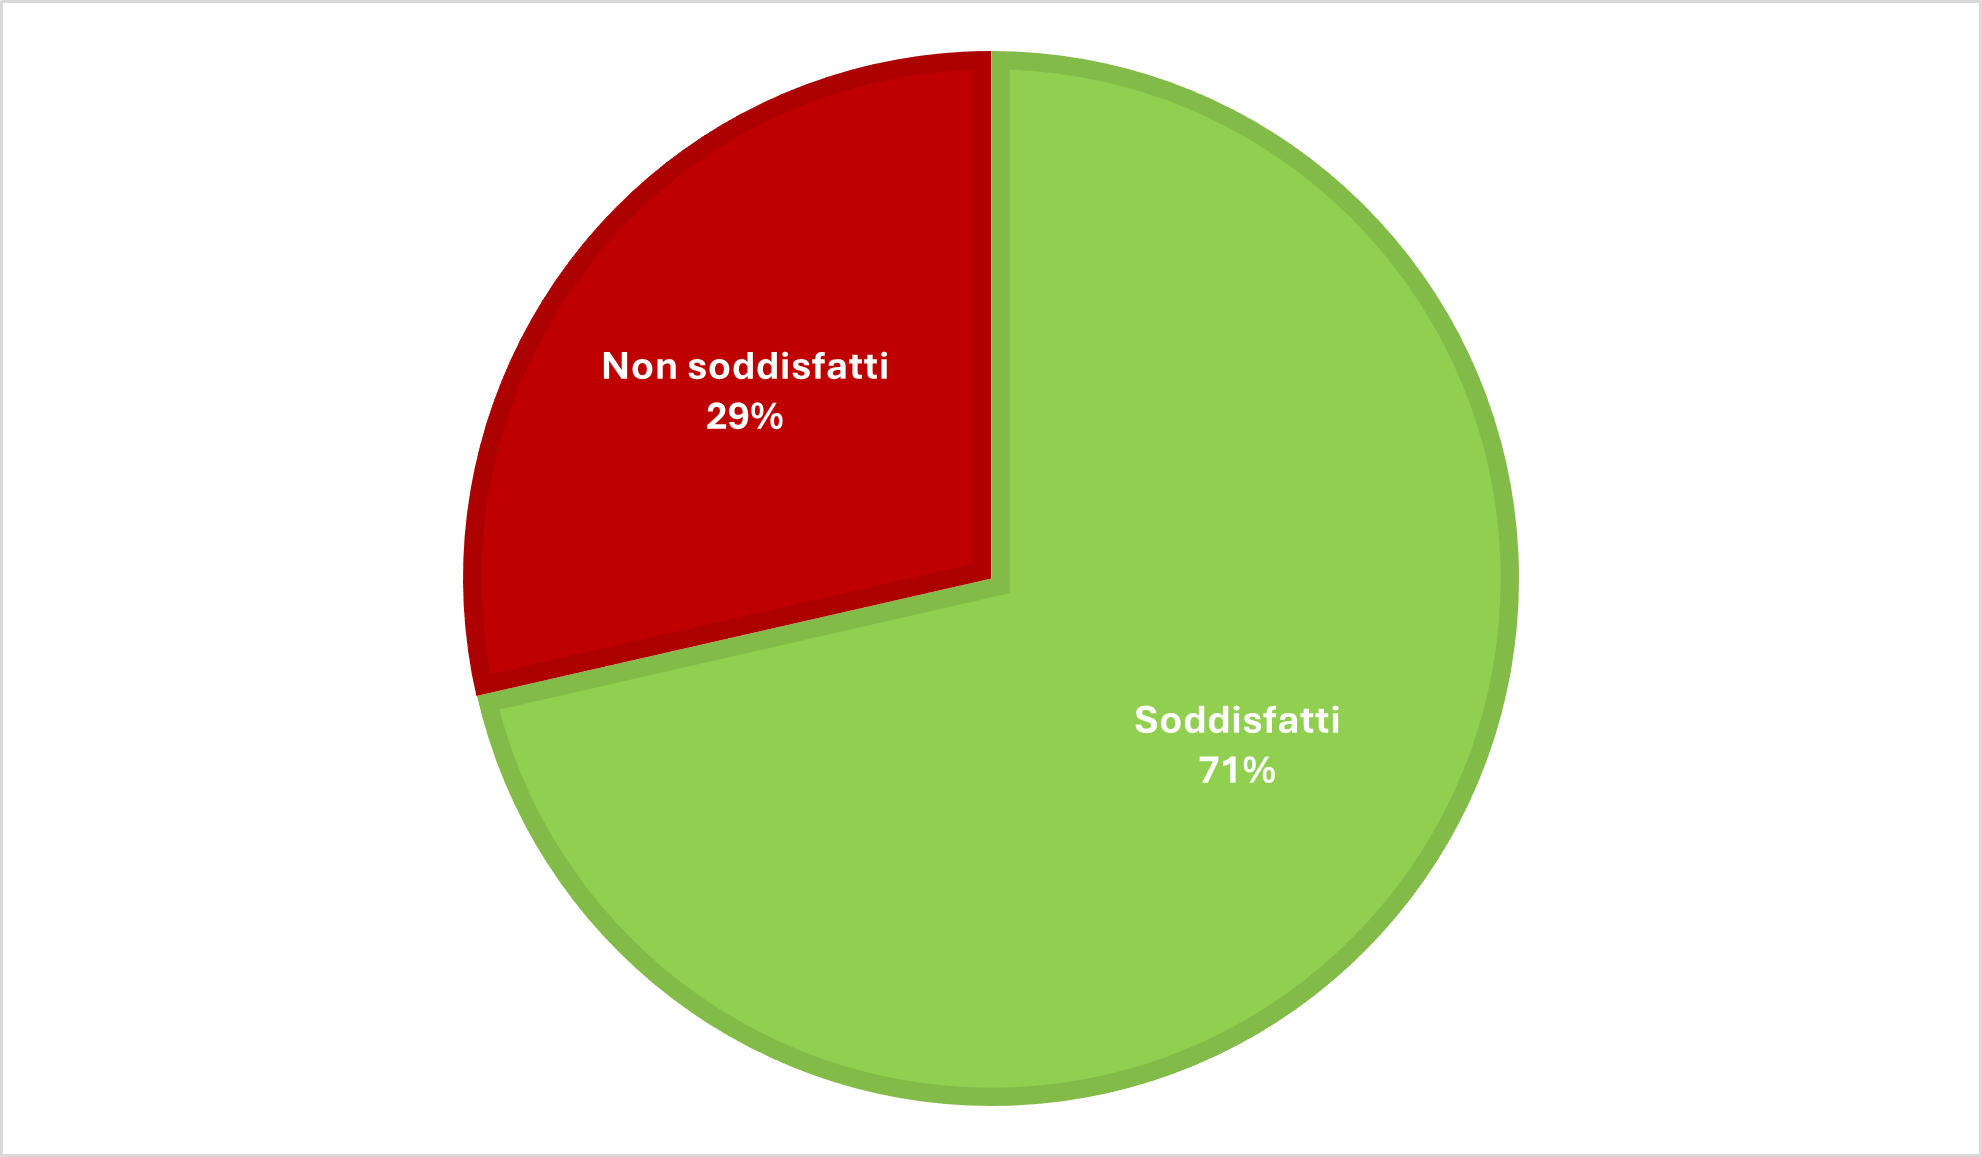
\includegraphics[width=0.7\textwidth]{images/stato_req_facolatativi.png}
    \caption{Grafico dello stato di copertura dei requisiti funzionali facoltativi}
\end{figure}


\newpage
%%%%%%%%%%%%%%%%%%%%%%%%%%%%%%%%%%%
% RIFERIMENTI ESTERNI
%%%%%%%%%%%%%%%%%%%%%%%%%%%%%%%%%%%
\section{Riferimenti esterni}\label{sec:ref_esterni}
Per ulteriori chiarimenti sugli argomenti discussi nel documento, si possono consultare i seguenti link esterni:
\begin{itemize}
    \item \textbf{Glossario v1.0.0}:\\
    \url{https://github.com/Avant-Garde-Software-Engineering/WMS3D/blob/main/Documentazione/PB/Esterna/glossario_v1.0.0.pdf}
    \item \textbf{Analisi dei requisiti v5.0.0}:\\
    \url{https://github.com/Avant-Garde-Software-Engineering/WMS3D/blob/main/Documentazione/PB/Esterna/analisi_dei_requisiti_v5.0.0.pdf}
    \item Capitolato \textbf{Warehouse Management 3D}:\\
    \url{https://www.math.unipd.it/~tullio/IS-1/2023/Progetto/C5.pdf} 
    \item Link alla \textbf{documentazione del gruppo}:\\
    \url{https://avant-garde-software-engineering.github.io/documentazione.html} \textcolor{gray}{\textit{(ultimo accesso 05-05-24)}}
\end{itemize}
Per riferimenti all'architettura e ai pattern adottati si possono consultare i link:
\begin{itemize}
    \item Link alla documentazione Zustand sulla \textbf{Flux inspired practice}:\\
    \url{https://docs.pmnd.rs/zustand/guides/flux-inspired-practice}
    \textcolor{gray}{\textit{(ultimo accesso 05-05-24)}}
    \item Link alla documentazione Zustand sullo \textbf{Slices pattern}:\\
    \url{https://docs.pmnd.rs/zustand/guides/slices-pattern}
    \textcolor{gray}{\textit{(ultimo accesso 05-05-24)}}
    \item Link alla documentazione Zustand su \textbf{Immutable state}:\\
    \url{https://docs.pmnd.rs/zustand/guides/immutable-state-and-merging}
    \textcolor{gray}{\textit{(ultimo accesso 05-05-24)}}
    \item Documentazione sull'\textbf{architettura a componenti} di React: \\
    \url{https://handsonreact.com/docs/component-architecture}
    \textcolor{gray}{\textit{(ultimo accesso 05-05-24)}}
    \item Documentazione sul \textbf{pattern Container/Presentational}:\\
    \url{https://www.patterns.dev/react/presentational-container-pattern/}
    \textcolor{gray}{\textit{(ultimo accesso 05-05-24)}}
\end{itemize}